%%%%%%%%%%%%%%%%%%%%%%%%%%%%%%%%%%%%%%%%%
% The Legrand Orange Book
% LaTeX Template
% Version 2.3 (8/8/17)
%
% This template has been downloaded from:
% http://www.LaTeXTemplates.com
%
% Original author:
% Mathias Legrand (legrand.mathias@gmail.com) with modifications by:
% Vel (vel@latextemplates.com)
%
% License:
% CC BY-NC-SA 3.0 (http://creativecommons.org/licenses/by-nc-sa/3.0/)
%
% Compiling this template:
% This template uses biber for its bibliography and makeindex for its index.
% When you first open the template, compile it from the command line with the 
% commands below to make sure your LaTeX distribution is configured correctly:
%
% 1) pdflatex main
% 2) makeindex main.idx -s StyleInd.ist
% 3) biber main
% 4) pdflatex main x 2
%
% After this, when you wish to update the bibliography/index use the appropriate
% command above and make sure to compile with pdflatex several times 
% afterwards to propagate your changes to the document.
%
% This template also uses a number of packages which may need to be
% updated to the newest versions for the template to compile. It is strongly
% recommended you update your LaTeX distribution if you have any
% compilation errors.
%
% Important note:
% Chapter heading images should have a 2:1 width:height ratio,
% e.g. 920px width and 460px height.
%
%%%%%%%%%%%%%%%%%%%%%%%%%%%%%%%%%%%%%%%%%

%----------------------------------------------------------------------------------------
%	PACKAGES AND OTHER DOCUMENT CONFIGURATIONS
%----------------------------------------------------------------------------------------

\documentclass[11pt,fleqn]{book} % Default font size and left-justified equations
%----------------------------------------------------------------------------------------

%%%%%%%%%%%%%%%%%%%%%%%%%%%%%%%%%%%%%%%%%
% The Legrand Orange Book
% Structural Definitions File
% Version 2.0 (9/2/15)
%
% Original author:
% Mathias Legrand (legrand.mathias@gmail.com) with modifications by:
% Vel (vel@latextemplates.com)
% 
% This file has been downloaded from:
% http://www.LaTeXTemplates.com
%
% License:
% CC BY-NC-SA 3.0 (http://creativecommons.org/licenses/by-nc-sa/3.0/)
%
%%%%%%%%%%%%%%%%%%%%%%%%%%%%%%%%%%%%%%%%%

%----------------------------------------------------------------------------------------
%	VARIOUS REQUIRED PACKAGES AND CONFIGURATIONS
%----------------------------------------------------------------------------------------
\usepackage[top=3cm,bottom=3cm,left=3cm,right=3cm,headsep=10pt,a4paper]{geometry} % Page margins
\usepackage[table]{xcolor}  % Required for specifying colors by name
\usepackage{graphicx} % Required for including pictures
\graphicspath{{Pictures/}} % Specifies the directory where pictures are stored

\usepackage{lipsum} % Inserts dummy text

\usepackage{wrapfig}

\usepackage{tikz} % Required for drawing custom shapes

\usepackage[dutch]{babel} % English language/hyphenation

\usepackage{enumitem} % Customize lists
\setlist{nolistsep} % Reduce spacing between bullet points and numbered lists

\usepackage{booktabs} % Required for nicer horizontal rules in tables

\usepackage{xcolor} % Required for specifying colors by name

\definecolor{ocre}{RGB}{0,161,255} % Define the orange color used for highlighting throughout the book
\definecolor{not}{RGB}{192,192,192} %


%----------------------------------------------------------------------------------------
%	FONTS
%----------------------------------------------------------------------------------------

\usepackage{avant} % Use the Avantgarde font for headings
%\usepackage{times} % Use the Times font for headings
\usepackage{mathptmx} % Use the Adobe Times Roman as the default text font together with math symbols from the Sym­bol, Chancery and Com­puter Modern fonts

\usepackage{microtype} % Slightly tweak font spacing for aesthetics
\usepackage[utf8]{inputenc} % Required for including letters with accents
\usepackage[T1]{fontenc} % Use 8-bit encoding that has 256 glyphs

%----------------------------------------------------------------------------------------
%	BIBLIOGRAPHY AND INDEX
%----------------------------------------------------------------------------------------

\usepackage[style=numeric,citestyle=numeric,sorting=none,sortcites=true,autopunct=true,babel=hyphen,hyperref=true,abbreviate=false,backref=true,backend=biber]{biblatex}
\addbibresource{bibliography.bib} % BibTeX bibliography file
\defbibheading{bibempty}{}

\usepackage{calc} % For simpler calculation - used for spacing the index letter headings correctly
\usepackage{makeidx} % Required to make an index
\makeindex % Tells LaTeX to create the files required for indexing

%----------------------------------------------------------------------------------------
%	MAIN TABLE OF CONTENTS
%----------------------------------------------------------------------------------------

\usepackage{titletoc} % Required for manipulating the table of contents

\contentsmargin{0cm} % Removes the default margin

% Part text styling
\titlecontents{part}[0cm]
{\addvspace{20pt}\centering\large\bfseries}
{}
{}
{}

% Chapter text styling
\titlecontents{chapter}[1.25cm] % Indentation
{\addvspace{12pt}\large\sffamily\bfseries} % Spacing and font options for chapters
{\color{ocre!60}\contentslabel[\Large\thecontentslabel]{1.25cm}\color{ocre}} % Chapter number
{\color{ocre}}  
{\color{ocre!60}\normalsize\;\titlerule*[.5pc]{.}\;\thecontentspage} % Page number

% Section text styling
\titlecontents{section}[1.25cm] % Indentation
{\addvspace{3pt}\sffamily\bfseries} % Spacing and font options for sections
{\contentslabel[\thecontentslabel]{1.25cm}} % Section number
{}
{\hfill\color{black}\thecontentspage} % Page number
[]

% Subsection text styling
\titlecontents{subsection}[1.25cm] % Indentation
{\addvspace{1pt}\sffamily\small} % Spacing and font options for subsections
{\contentslabel[\thecontentslabel]{1.25cm}} % Subsection number
{}
{\ \titlerule*[.5pc]{.}\;\thecontentspage} % Page number
[]

% List of figures
\titlecontents{figure}[0em]
{\addvspace{-5pt}\sffamily}
{\thecontentslabel\hspace*{1em}}
{}
{\ \titlerule*[.5pc]{.}\;\thecontentspage}
[]

% List of tables
\titlecontents{table}[0em]
{\addvspace{-5pt}\sffamily}
{\thecontentslabel\hspace*{1em}}
{}
{\ \titlerule*[.5pc]{.}\;\thecontentspage}
[]

%----------------------------------------------------------------------------------------
%	MINI TABLE OF CONTENTS IN PART HEADS
%----------------------------------------------------------------------------------------

\titlecontents{lchapter}[0em] % Indenting
{\addvspace{15pt}\large\sffamily\bfseries} % Spacing and font options for chapters
{\color{ocre}\contentslabel[\Large\thecontentslabel]{1.25cm}\color{ocre}} % Chapter number
{}  
{\color{ocre}\normalsize\sffamily\bfseries\;\titlerule*[.5pc]{.}\;\thecontentspage} % Page number

% Section text styling
\titlecontents{lsection}[0em] % Indenting
{\sffamily\small} % Spacing and font options for sections
{\contentslabel[\thecontentslabel]{1.25cm}} % Section number
{}
{}

% Subsection text styling
\titlecontents{lsubsection}[.5em] % Indentation
{\normalfont\footnotesize\sffamily} % Font settings
{}
{}
{}

%----------------------------------------------------------------------------------------
%	PAGE HEADERS
%----------------------------------------------------------------------------------------

\usepackage{fancyhdr} % Required for header and footer configuration

\pagestyle{fancy}
\renewcommand{\chaptermark}[1]{\markboth{\sffamily\normalsize\bfseries\chaptername\ \thechapter.\ #1}{}} % Chapter text font settings
\renewcommand{\sectionmark}[1]{}
%\renewcommand{\sectionmark}[1]{\markright{\sffamily\normalsize\thesection\hspace{5pt}#1}{}} % Section text font settings
%\fancyhf{} \fancyhead[LE,RO]{\sffamily\normalsize\thepage} %removed by CP
\fancyhf{} \fancyhead[LE,RO]{\sffamily\normalsize} % Font setting for the page number in the header
\fancyhead[LO]{\rightmark} % Print the nearest section name on the left side of odd pages
\fancyhead[RE]{\leftmark} % Print the current chapter name on the right side of even pages
\fancyfoot[LE,RO]{\sffamily\normalsize\thepage} %added by CP
%\fancyfoot[C]{CONCEPT VERSIE}
\renewcommand{\headrulewidth}{0.5pt} % Width of the rule under the header
\addtolength{\headheight}{2.5pt} % Increase the spacing around the header slightly
\renewcommand{\footrulewidth}{0pt} % Removes the rule in the footer
\fancypagestyle{plain}{\fancyhead{}\renewcommand{\headrulewidth}{0pt}} % Style for when a plain pagestyle is specified

% Removes the header from odd empty pages at the end of chapters
\makeatletter
\renewcommand{\cleardoublepage}{
\clearpage\ifodd\c@page\else
\hbox{}
\vspace*{\fill}
\thispagestyle{empty}
\newpage
\fi}

%----------------------------------------------------------------------------------------
%	THEOREM STYLES
%----------------------------------------------------------------------------------------

\usepackage{amsmath,amsfonts,amssymb,amsthm} % For math equations, theorems, symbols, etc

\newcommand{\intoo}[2]{\mathopen{]}#1\,;#2\mathclose{[}}
\newcommand{\ud}{\mathop{\mathrm{{}d}}\mathopen{}}
\newcommand{\intff}[2]{\mathopen{[}#1\,;#2\mathclose{]}}
\newtheorem{notation}{Notation}[chapter]

% Boxed/framed environments
\newtheoremstyle{ocrenumbox}% % Theorem style name
{0pt}% Space above
{0pt}% Space below
{\normalfont}% % Body font
{}% Indent amount
{\small\bf\sffamily\color{ocre}}% % Theorem head font
{\;}% Punctuation after theorem head
{0.25em}% Space after theorem head
{\small\sffamily\color{ocre}\thmname{#1}\nobreakspace\thmnumber{\@ifnotempty{#1}{}\@upn{#2}}% Theorem text (e.g. Theorem 2.1)
\thmnote{\nobreakspace\the\thm@notefont\sffamily\bfseries\color{black}---\nobreakspace#3.}} % Optional theorem note
\renewcommand{\qedsymbol}{$\blacksquare$}% Optional qed square

\newtheoremstyle{blacknumex}% Theorem style name
{5pt}% Space above
{5pt}% Space below
{\normalfont}% Body font
{} % Indent amount
{\small\bf\sffamily}% Theorem head font
{\;}% Punctuation after theorem head
{0.25em}% Space after theorem head
{\small\sffamily{\tiny\ensuremath{\blacksquare}}\nobreakspace\thmname{#1}\nobreakspace\thmnumber{\@ifnotempty{#1}{}\@upn{#2}}% Theorem text (e.g. Theorem 2.1)
\thmnote{\nobreakspace\the\thm@notefont\sffamily\bfseries---\nobreakspace#3.}}% Optional theorem note

\newtheoremstyle{blacknumbox} % Theorem style name
{0pt}% Space above
{0pt}% Space below
{\normalfont}% Body font
{}% Indent amount
{\small\bf\sffamily}% Theorem head font
{\;}% Punctuation after theorem head
{0.25em}% Space after theorem head
{\small\sffamily\thmname{#1}\nobreakspace\thmnumber{\@ifnotempty{#1}{}\@upn{#2}}% Theorem text (e.g. Theorem 2.1)
\thmnote{\nobreakspace\the\thm@notefont\sffamily\bfseries---\nobreakspace#3.}}% Optional theorem note

% Non-boxed/non-framed environments
\newtheoremstyle{ocrenum}% % Theorem style name
{5pt}% Space above
{5pt}% Space below
{\normalfont}% % Body font
{}% Indent amount
{\small\bf\sffamily\color{ocre}}% % Theorem head font
{\;}% Punctuation after theorem head
{0.25em}% Space after theorem head
{\small\sffamily\color{ocre}\thmname{#1}\nobreakspace\thmnumber{\@ifnotempty{#1}{}\@upn{#2}}% Theorem text (e.g. Theorem 2.1)
\thmnote{\nobreakspace\the\thm@notefont\sffamily\bfseries\color{black}---\nobreakspace#3.}} % Optional theorem note
\renewcommand{\qedsymbol}{$\blacksquare$}% Optional qed square
\makeatother

% Defines the theorem text style for each type of theorem to one of the three styles above
\newcounter{dummy} 
\numberwithin{dummy}{section}
\theoremstyle{ocrenumbox}
\newtheorem{theoremeT}[dummy]{Theorem}
\newtheorem{problem}{Problem}[chapter]
\newtheorem{exerciseT}{Exercise}[chapter]
\theoremstyle{blacknumex}
\newtheorem{exampleT}{Example}[chapter]
\theoremstyle{blacknumbox}
\newtheorem{vocabulary}{Vocabulary}[chapter]
\newtheorem{definitionT}{Definition}[section]
\newtheorem{corollaryT}[dummy]{Corollary}
\theoremstyle{ocrenum}
\newtheorem{proposition}[dummy]{Proposition}

%----------------------------------------------------------------------------------------
%	DEFINITION OF COLORED BOXES
%----------------------------------------------------------------------------------------

\RequirePackage[framemethod=default]{mdframed} % Required for creating the theorem, definition, exercise and corollary boxes

% Theorem box
\newmdenv[skipabove=7pt,
skipbelow=7pt,
backgroundcolor=black!5,
linecolor=ocre,
innerleftmargin=5pt,
innerrightmargin=5pt,
innertopmargin=5pt,
leftmargin=0cm,
rightmargin=0cm,
innerbottommargin=5pt]{tBox}

% Exercise box	  
\newmdenv[skipabove=7pt,
skipbelow=7pt,
rightline=false,
leftline=true,
topline=false,
bottomline=false,
backgroundcolor=ocre!10,
linecolor=ocre,
innerleftmargin=5pt,
innerrightmargin=5pt,
innertopmargin=5pt,
innerbottommargin=5pt,
leftmargin=0cm,
rightmargin=0cm,
linewidth=4pt]{eBox}	

% Definition box
\newmdenv[skipabove=7pt,
skipbelow=7pt,
rightline=false,
leftline=true,
topline=false,
bottomline=false,
linecolor=ocre,
innerleftmargin=5pt,
innerrightmargin=5pt,
innertopmargin=0pt,
leftmargin=0cm,
rightmargin=0cm,
linewidth=4pt,
innerbottommargin=0pt]{dBox}	

% Corollary box
\newmdenv[skipabove=7pt,
skipbelow=7pt,
rightline=false,
leftline=true,
topline=false,
bottomline=false,
linecolor=gray,
backgroundcolor=black!5,
innerleftmargin=5pt,
innerrightmargin=5pt,
innertopmargin=5pt,
leftmargin=0cm,
rightmargin=0cm,
linewidth=4pt,
innerbottommargin=5pt]{cBox}

% Creates an environment for each type of theorem and assigns it a theorem text style from the "Theorem Styles" section above and a colored box from above
\newenvironment{theorem}{\begin{tBox}\begin{theoremeT}}{\end{theoremeT}\end{tBox}}
\newenvironment{exercise}{\begin{eBox}\begin{exerciseT}}{\hfill{\color{ocre}\tiny\ensuremath{\blacksquare}}\end{exerciseT}\end{eBox}}				  
\newenvironment{definition}{\begin{dBox}\begin{definitionT}}{\end{definitionT}\end{dBox}}	
\newenvironment{example}{\begin{exampleT}}{\hfill{\tiny\ensuremath{\blacksquare}}\end{exampleT}}		
\newenvironment{corollary}{\begin{cBox}\begin{corollaryT}}{\end{corollaryT}\end{cBox}}	

%----------------------------------------------------------------------------------------
%	REMARK ENVIRONMENT
%----------------------------------------------------------------------------------------

\newenvironment{remark}{\par\vspace{10pt}\small % Vertical white space above the remark and smaller font size
\begin{list}{}{
\leftmargin=35pt % Indentation on the left
\rightmargin=25pt}\item\ignorespaces % Indentation on the right
\makebox[-2.5pt]{\begin{tikzpicture}[overlay]
\node[draw=ocre!60,line width=1pt,circle,fill=ocre!25,font=\sffamily\bfseries,inner sep=2pt,outer sep=0pt] at (-15pt,0pt){\textcolor{ocre}{R}};\end{tikzpicture}} % Orange R in a circle
\advance\baselineskip -1pt}{\end{list}\vskip5pt} % Tighter line spacing and white space after remark

%----------------------------------------------------------------------------------------
%	SECTION NUMBERING IN THE MARGIN
%----------------------------------------------------------------------------------------

\makeatletter
\renewcommand{\@seccntformat}[1]{\llap{\textcolor{ocre}{\csname the#1\endcsname}\hspace{1em}}}                    
\renewcommand{\section}{\@startsection{section}{1}{\z@}
{-4ex \@plus -1ex \@minus -.4ex}
{1ex \@plus.2ex }
{\normalfont\large\sffamily\bfseries}}
\renewcommand{\subsection}{\@startsection {subsection}{2}{\z@}
{-3ex \@plus -0.1ex \@minus -.4ex}
{0.5ex \@plus.2ex }
{\normalfont\sffamily\bfseries}}
\renewcommand{\subsubsection}{\@startsection {subsubsection}{3}{\z@}
{-2ex \@plus -0.1ex \@minus -.2ex}
{.2ex \@plus.2ex }
{\normalfont\small\sffamily\bfseries}}                        
\renewcommand\paragraph{\@startsection{paragraph}{4}{\z@}
{-2ex \@plus-.2ex \@minus .2ex}
{.1ex}
{\normalfont\small\sffamily\bfseries}}

%----------------------------------------------------------------------------------------
%	PART HEADINGS
%----------------------------------------------------------------------------------------

% numbered part in the table of contents
\newcommand{\@mypartnumtocformat}[2]{%
\setlength\fboxsep{0pt}%
\noindent\colorbox{ocre!20}{\strut\parbox[c][.7cm]{\ecart}{\color{ocre!70}\Large\sffamily\bfseries\centering#1}}\hskip\esp\colorbox{ocre!40}{\strut\parbox[c][.7cm]{\linewidth-\ecart-\esp}{\Large\sffamily\centering#2}}}%
%%%%%%%%%%%%%%%%%%%%%%%%%%%%%%%%%%
% unnumbered part in the table of contents
\newcommand{\@myparttocformat}[1]{%
\setlength\fboxsep{0pt}%
\noindent\colorbox{ocre!40}{\strut\parbox[c][.7cm]{\linewidth}{\Large\sffamily\centering#1}}}%
%%%%%%%%%%%%%%%%%%%%%%%%%%%%%%%%%%
\newlength\esp
\setlength\esp{4pt}
\newlength\ecart
\setlength\ecart{1.2cm-\esp}
\newcommand{\thepartimage}{}%
\newcommand{\partimage}[1]{\renewcommand{\thepartimage}{#1}}%
\def\@part[#1]#2{%
\ifnum \c@secnumdepth >-2\relax%
\refstepcounter{part}%
\addcontentsline{toc}{part}{\texorpdfstring{\protect\@mypartnumtocformat{\thepart}{#1}}{\partname~\thepart\ ---\ #1}}
\else%
\addcontentsline{toc}{part}{\texorpdfstring{\protect\@myparttocformat{#1}}{#1}}%
\fi%
\startcontents%
\markboth{}{}%
{\thispagestyle{empty}%
\begin{tikzpicture}[remember picture,overlay]%
\node at (current page.north west){\begin{tikzpicture}[remember picture,overlay]%	
\fill[ocre!20](0cm, 0cm) rectangle (\paperwidth,-\paperheight);
\node[anchor=north] at (4cm,-3.25cm){\color{ocre!40}\fontsize{220}{100}\sffamily\bfseries\thepart}; 

\ifnum \value{part}=1 %added by CP. If first chapter
\node[anchor=south east] at (\paperwidth-1cm,-\paperheight+2.5cm){\parbox[t][][t]{8.5cm}{
		\printcontents{l}{0}{\setcounter{tocdepth}{1}}%
}};

\makeatletter
\newcommand \Dotfill {\leavevmode \cleaders \hb@xt@ .22cm{\hss .\hss }\hfill \kern \z@}
\makeatother
\node[anchor=south east] at (\paperwidth-1cm,-\paperheight+1cm) {\parbox[t][][t]{10cm}{
		\large\sffamily\bfseries\large \color{ocre}
		\begin{tabular}{p{0.9cm} p{8.5cm}}
		\Large II & \hyperref[part:oefen]{Oefenvragen} \normalsize\Dotfill \vspace{0.05cm} \hspace{0.05cm} \pageref{part:oefen} \\ 
		\Large III & \hyperref[part:manoeuvre]{Zeilmanoeuvres} \normalsize\Dotfill \hspace{0.05cm} \pageref{part:manoeuvre}
		\end{tabular}
}}; 
\else
\node[anchor=south east] at (\paperwidth-1cm,-\paperheight+1cm){\parbox[t][][t]{8.5cm}{
		\printcontents{l}{0}{\setcounter{tocdepth}{1}}%
}};
\fi %added by CP. If first chapter



\node[anchor=north east] at (\paperwidth-1.5cm,-3.25cm){\parbox[t][][t]{15cm}{\strut\raggedleft\color{white}\fontsize{30}{30}\sffamily\bfseries#2}};
\end{tikzpicture}};
\end{tikzpicture}}%
\@endpart}
\def\@spart#1{%
\startcontents%
\phantomsection
{\thispagestyle{empty}%
\begin{tikzpicture}[remember picture,overlay]%
\node at (current page.north west){\begin{tikzpicture}[remember picture,overlay]%	
\fill[ocre!20](0cm,0cm) rectangle (\paperwidth,-\paperheight);
\node[anchor=north east] at (\paperwidth-1.5cm,-3.25cm){\parbox[t][][t]{15cm}{\strut\raggedleft\color{white}\fontsize{30}{30}\sffamily\bfseries#1}};
\end{tikzpicture}};
\end{tikzpicture}}
\addcontentsline{toc}{part}{\texorpdfstring{%
\setlength\fboxsep{0pt}%
\noindent\protect\colorbox{ocre!40}{\strut\protect\parbox[c][.7cm]{\linewidth}{\Large\sffamily\protect\centering #1\quad\mbox{}}}}{#1}}%
\@endpart}
\def\@endpart{\vfil\newpage
\if@twoside
\if@openright
\null
\thispagestyle{empty}%
\newpage
\fi
\fi
\if@tempswa
\twocolumn
\fi}

%----------------------------------------------------------------------------------------
%	CHAPTER HEADINGS
%----------------------------------------------------------------------------------------

% A switch to conditionally include a picture, implemented by  Christian Hupfer
\newif\ifusechapterimage
\usechapterimagetrue
\newcommand{\thechapterimage}{}%
\newcommand{\chapterimage}[1]{\ifusechapterimage\renewcommand{\thechapterimage}{#1}\fi}%
\newcommand{\autodot}{.}
\def\@makechapterhead#1{%
{\parindent \z@ \raggedright \normalfont
\ifnum \c@secnumdepth >\m@ne
\if@mainmatter
\begin{tikzpicture}[remember picture,overlay]
\node at (current page.north west)
{\begin{tikzpicture}[remember picture,overlay]
\node[anchor=north west,inner sep=0pt] at (0,0) {\ifusechapterimage\includegraphics[width=\paperwidth]{\thechapterimage}\fi};
%\textbf{\draw[anchor=west] (0cm,-4.6cm) node [fill=black,fill opacity=0.4,inner sep=12pt]{\strut\makebox[22cm]{}};}

%added by christian
{\ifusechapterimage
\textbf{\draw[anchor=west] (0cm,-4.6cm) node [fill=black,fill opacity=0.4,inner sep=12pt]{\strut\makebox[22cm]{}};}
\draw[anchor=west] (1.5cm,-4.7cm) node {\Huge\sffamily\bfseries\color{white}\thechapter\autodot~#1\strut};
\else 
\textbf{\draw[anchor=west] (0cm,-1cm) node [fill=black,fill opacity=0.4,inner sep=12pt]{\strut\makebox[22cm]{}};}
\draw[anchor=west] (1.5cm,-1.1cm) node {\Huge\sffamily\bfseries\color{white}\thechapter\autodot~#1\strut};
\fi};

%\draw[anchor=west] (1.5cm,-4.7cm) node {\Huge\sffamily\bfseries\color{white}\thechapter\autodot~#1\strut};
\end{tikzpicture}};
\end{tikzpicture}
\else
\begin{tikzpicture}[remember picture,overlay]
\node at (current page.north west)
{\begin{tikzpicture}[remember picture,overlay]
\node[anchor=north west,inner sep=0pt] at (0,0) {\ifusechapterimage\includegraphics[width=\paperwidth]{\thechapterimage}\fi};
\draw[anchor=west] (10.1cm,-10.02cm) node {\Huge\sffamily\bfseries\color{white}#1\strut};
\end{tikzpicture}};
\end{tikzpicture}
\fi\fi\par\vspace*{100\p@}}}

%-------------------------------------------

\def\@makeschapterhead#1{%
\begin{tikzpicture}[remember picture,overlay]
\node at (current page.north west)
{\begin{tikzpicture}[remember picture,overlay]
\node[anchor=north west,inner sep=0pt] at (0,0) {\ifusechapterimage\includegraphics[width=\paperwidth]{\thechapterimage}\fi};
\draw[anchor=west] (13cm,-10.02cm) node {\Huge\sffamily\bfseries\color{white}#1\strut};
\end{tikzpicture}};
\end{tikzpicture}
\par\vspace*{230\p@}}
\makeatother

%----------------------------------------------------------------------------------------
%	HYPERLINKS IN THE DOCUMENTS
%----------------------------------------------------------------------------------------

\usepackage{hyperref}
\hypersetup{hidelinks,backref=true,pagebackref=true,hyperindex=true,colorlinks=false,breaklinks=true,urlcolor= ocre,bookmarks=true,bookmarksopen=false,
	pdftitle={Kielboot II - Scouting Sint Maarten},
	pdfauthor={Christian Peppelman},
	pdfsubject={Kielboot II - Zeiltheorie met focus op Scouting},
	pdfkeywords={CWO Kielboot II},
}
\usepackage{bookmark}
\bookmarksetup{
open,
numbered,
addtohook={%
\ifnum\bookmarkget{level}=0 % chapter
\bookmarksetup{bold}%
\fi
\ifnum\bookmarkget{level}=-1 % part
\bookmarksetup{color=ocre,bold}%
\fi
}
}

%----------------------------------------------------------------------------------------
%	Excercises
%----------------------------------------------------------------------------------------
\newcommand{\question}[2]{{\sffamily\bfseries{\textcolor{ocre}{\hspace{-0.5cm}#1. }{#2}}}}

\newcommand{\answerTextFour}[4]{
\begin{enumerate}[topsep=-2pt, label=\Alph*.]
    \item #1
    \item #2
    \item #3
    \item #4
\end{enumerate}}


\newcommand{\answerTextPicture}[5]{
\begin{figure}[H]	
	\vspace{-10px}
     \begin{minipage}[]{0.70\textwidth}
        \begin{enumerate}[topsep=0pt, label=\Alph*.]
            \item #1
            \item #2
            \item #3
            \item #4
        \end{enumerate}
      \end{minipage}
      \begin{minipage}[]{0.29\textwidth}
            \begin{figure}[H]
            \includegraphics[width=0.80\textwidth,right]{#5}
            \end{figure}
      \end{minipage}
  \vspace{-10px}
\end{figure}
}

\newcommand{\answerPicture}[4]{
\begin{figure}[H]
  \centering
  \begin{minipage}[b]{0.23\textwidth}
    \includegraphics[width=\textwidth]{#1}
    \centering
    A
  \end{minipage}
  \hfill
  \begin{minipage}[b]{0.23\textwidth}
    \includegraphics[width=\textwidth]{#2}
    \centering
    B
  \end{minipage}
  \hfill
  \begin{minipage}[b]{0.23\textwidth}
    \includegraphics[width=\textwidth]{#3}
    \centering
    C
  \end{minipage}
  \hfill
  \begin{minipage}[b]{0.23\textwidth}
    \includegraphics[width=\textwidth]{#4}
    \centering
    D
  \end{minipage}
\end{figure}
} % Insert the commands.tex file which contains the majority of the structure behind the template
\usepackage{graphicx}
\usepackage{lscape}
\usepackage{pgfgantt}
\usepackage{multicol}
\usepackage{caption} 
\usepackage{float}
\usepackage{pdfpages}
\usepackage{wrapfig}
\usepackage{enumitem}
\usepackage[export]{adjustbox}
\captionsetup[table]{skip=5pt}
\usepackage{parskip} %CP
\usepackage{geometry} %for margin notes
\usepackage{marginnote} %for margin notes
\usepackage{array}
\usepackage{multirow}

\pdfinclusioncopyfonts=1 % This fixes missing characher form figures
\pdfsuppresswarningpagegroup=1 % ignore page group warning

%Header and front folder selection

%%% Sint Maarten %%%
\newcommand{\header}[1]{\chapterimage{Banners/header_#1.png}}
\newcommand{\omslag}{Omslag/omslag.pdf}

\begin{document}

%----------------------------------------------------------------------------------------
%	TITLE PAGE
%----------------------------------------------------------------------------------------

\begingroup
\thispagestyle{empty}
\begin{tikzpicture}[remember picture,overlay]
\node[inner sep=0pt] (background) at (current page.center) {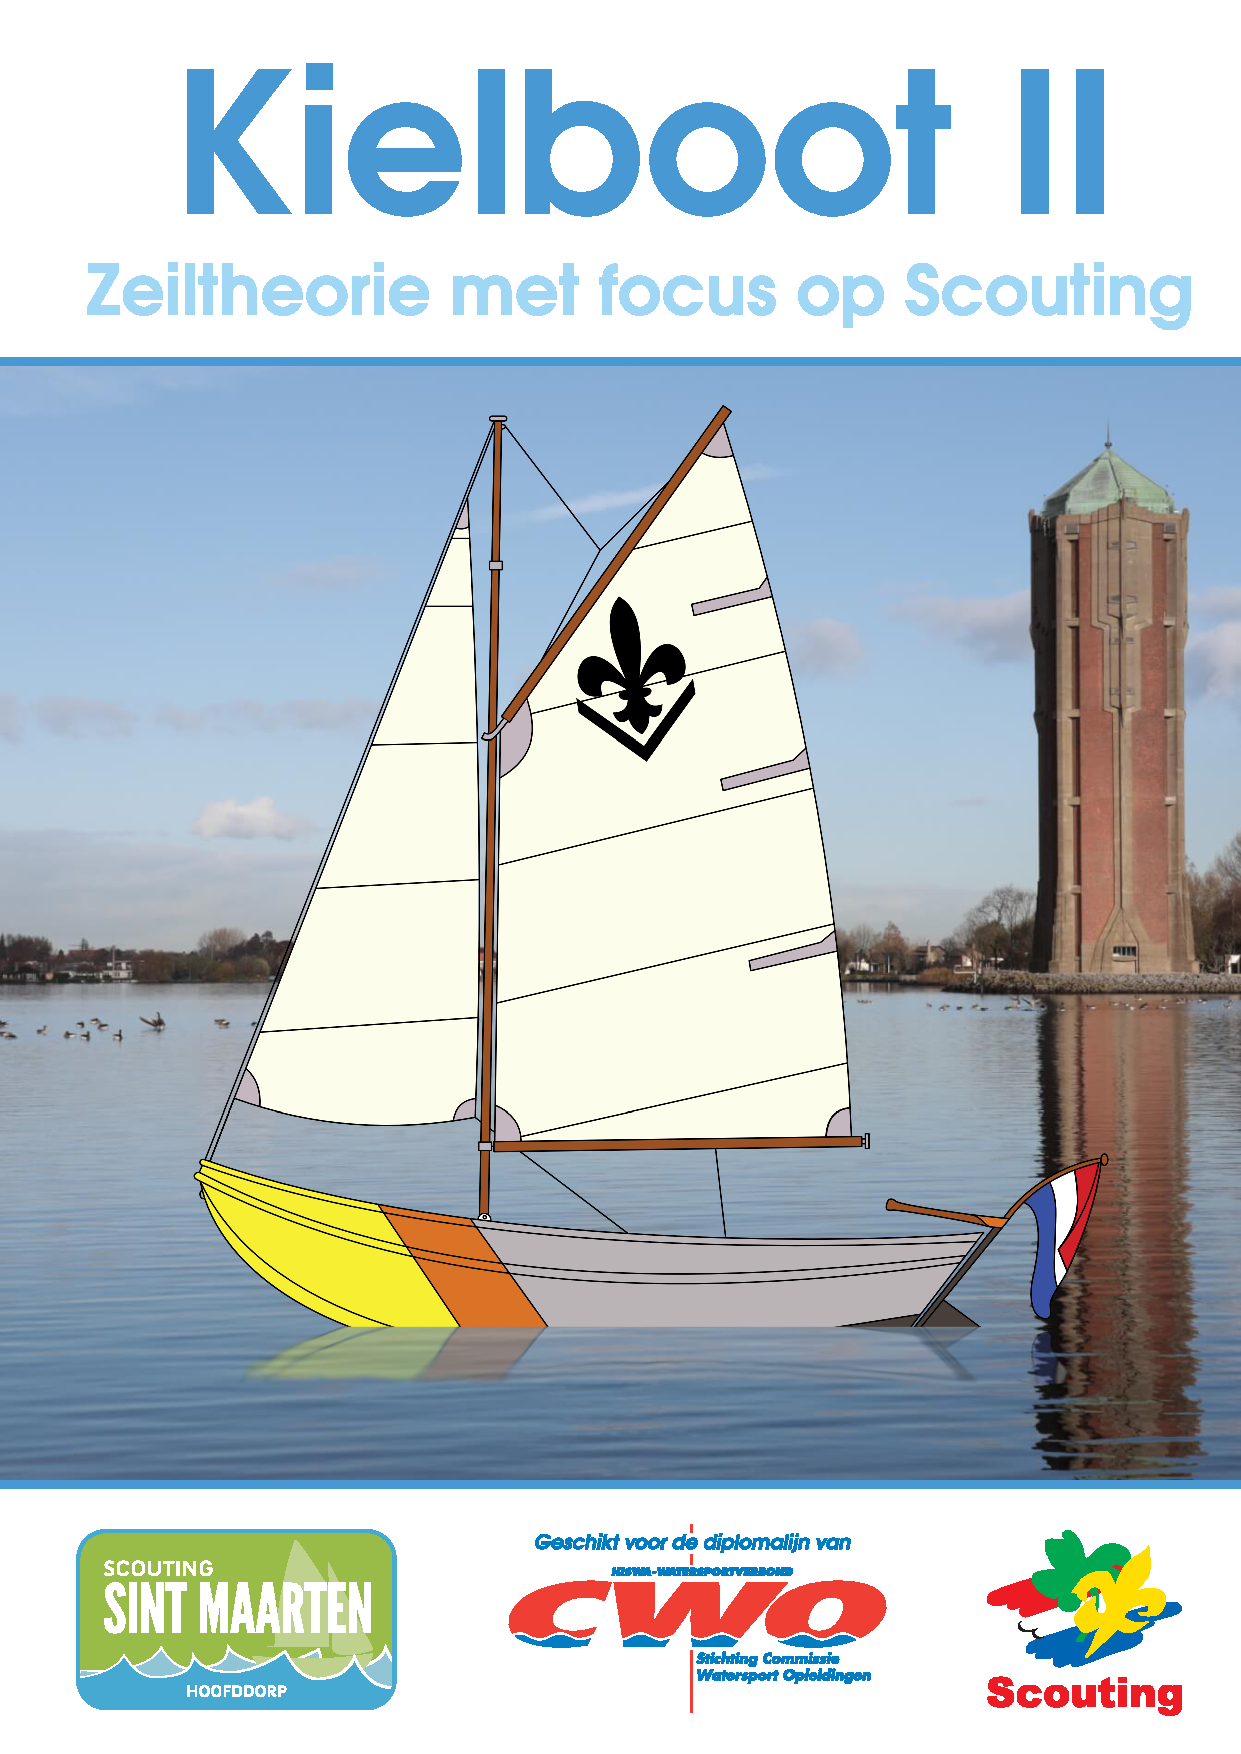
\includegraphics[width=\paperwidth, page = 1]{\omslag}};
\end{tikzpicture}
\vfill
\endgroup

%----------------------------------------------------------------------------------------
%	COPYRIGHT PAGE
%----------------------------------------------------------------------------------------

\newpage
{\sffamily\bfseries Naam: }\rule{60mm}{.1pt}%
~\vfill
\thispagestyle{empty}
Voorpagina ontworpen door Christian Peppelman 2021. Achtergrond foto: Visit Aalsmeer. Website: \url{https://www.visitaalsmeer.nl/10x-weetjes-de-westeinderplassen/}. Tekening lelievlet gebaseerd op \textit{CWO Instructieboek} van de Katwijkse Zeeverkenners (zie dankwoord). 
Handelsmerken op het voorblad zijn van respectievelijke stichtingen of organisaties. De CWO en Scouting Nederland zijn niet betrokken geweest bij het opstellen van dit lesboek.

\textit{Opgeleverd op \today} % Printing/edition date


\header{0}
\chapter*{Voorwoord}

\section{Voorwoord}
Om ons huidige, inmiddels flink verouderde, kielboot theorieboek te vervangen ben ik begin 2018 begonnen met het schrijven van deze vernieuwde versie. Hoewel het oude boek zeker niet slecht was, was het duidelijk tijd voor wat vernieuwing. Qua inhoud is dit boek erg geïnspireerd op zijn voorloper, met de onderscheidende factor van duidelijkere afbeeldingen en illustraties, verbeterde teksten en een modern thema.

- Christian Peppelman
\section{Dankwoord}
Tijdens het opstellen van dit boek heb ik heel erg veel waardevolle feedback mogen ontvangen van medeleden van onze scoutingvereniging. Ik wil hen daar hartelijk voor bedanken! In het bijzonder Yara, Robert en Wouter voor de kritische, maar opbouwende feedback die dit boek gemaakt heeft tot wat het nu is.\\
Daarnaast wil ik ook graag de Katwijkse Zeeverkenners bedanken voor het online beschikbaar stellen van hun uitstekende lesboeken (\url{https://www.katwijksezeeverkenners.nl/cwo/instructieboeken/}). Het lesboek van de Katwijkse Zeeverkenners is een grote inspiratiebron geweest voor de figuren in dit lesboek.

\newpage
\section{Lesstof verantwoording}
De lesstof die in dit boek aan bod komt, is gemaakt om aan de eisen van de stichting Commissie Watersport Opleidingen (CWO) te voldoen voor de discipline kielboot II. Deze eisen zijn te vinden op \url{https://cwo.nl/leren-varen/kielboot}. Op sommige vlakken gaat dit boek uitgebreider in op de stof dan vanuit het CWO strikt noodzakelijk is. Hiervoor is gekozen omdat deze kennis een toegevoegde waarde kan bieden tijdens het zeilen op scouting.


\section{Document Informatie}
\subsection*{Licentie}
\begin{figure}[H]
	\centering
	\begin{minipage}[t]{0.60\textwidth}
		\vspace{-1.80cm}
		Dit boek is uitgebracht onder een Creative Commons
		'Naamsvermelding-NietCommercieel-GelijkDelen 4.0 Internationaal' (CC BY-NC-SA 4.0) licentie. Voor meer informatie: \url{https://creativecommons.org/licenses/by-nc-sa/4.0/}
	\end{minipage}
	\hfill
	\begin{minipage}[b]{0.35\textwidth}
	
\includegraphics[width=\textwidth]{../Hoofdstukken/Informatie/CC-BY-NC-SA.png}
\end{minipage}
\end{figure}
\subsection*{Auteur informatie}
Dit boek is geschreven door Christian Peppelman.\\ 
Voor contact, vragen of verbeteringen kun je mailen naar: \href{mailto:cwo@sintmaartengroep.nl}{CWO@sintmaartengroep.nl} 
\subsection*{Gebruik}
Om optimaal gebruik te kunnen maken van dit lesboek, deze graag laten drukken in een geniete brochure in kleur. Gelieve het boek niet thuis te printen, inscannen of vermenigvuldigen in een manier die negatieve invloed op de kwaliteit heeft. Voor de originele bestanden of gedrukte varianten kun je contact opnemen of kijken op \url{https://sintmaartengroep.nl/}
\subsection*{Thema}
Het thema waar dit boek op gebaseerd is heet `The Legrand Orange Book' en is ontworpen door Mathias Legrand. Het thema is gedownload op \url{https://nl.overleaf.com/latex/templates/} en valt onder een Creative Commons BY-NC-SA 3.0 licentie.
\subsection*{Versiebeheer}
\begin{table}[H]
	\centering
	\begin{tabular}{c|l|p{8cm}}
		\textbf{Versie} & \textbf{Datum} & \textbf{Omschrijving} \\ \hline
		1.5 & 9 januari 2019 & Eerste druk  \\ \hline
	    1.6 & 23 augustus 2019 & Toevoeging Deel III: Zeilmanoeuvres  \\ \hline
		1.7 & 24 september 2019  & Spelling verbeteringen \\ \hline
		2.0 & 5 januari 2020  & Afronding versie 2 \\ \hline
		2.1 & 21 maart 2020  & Kleine verbeteringen \\ \hline
		2.2 & 23 maart 2021  & Figuur 2.5 vernieuwd en toevoeging antwoordenblad \\ \hline	
		2.3 & 6 november 2023  & Update hoofdstuk reglementen
	\end{tabular}
\end{table}


\textit{Versie 2.3 \hspace{1 cm} 6 november 2023}
%Druk verhoogt alleen met 0.x versie verhogingen of hoger

%----------------------------------------------------------------------------------------
%	TABLE OF CONTENTS
%----------------------------------------------------------------------------------------

%\usechapterimagefalse % If you don't want to include a chapter image, use this to toggle images off - it can be enabled later with \usechapterimagetrue

\pagestyle{empty} % No headers

%\tableofcontents % Print the table of contents itself

%\cleardoublepage % Forces the first chapter to start on an odd page so it's on the right

\pagestyle{fancy} % Print headers again
\part{Theorie Lessen}
\header{2}
\chapter{Bootonderdelen \& Zeiltermen}
\section{Inleiding}
In dit hoofdstuk komen de verschillende onderdelen van de boot en een aantal zeiltermen aan bod. Deze termen en onderdelen zijn belangrijk om de volgende hoofdstukken in dit boek goed te begrijpen.

\section{Zeiltermen}
Voor duidelijke communicatie tijdens de les en in de boot is het van belang dat je een aantal zeiltermen kent. De belangrijkste termen worden hieronder besproken.

\subsection{Bakboord, Stuurboord, Loef en Lij}
Bakboord en stuurboord zijn het links en rechts \textbf{van de boot}, gezien vanaf het achterdek. Je moet altijd met de vaarrichting mee kijken. 

Loef en lij zeggen iets over de wind ten opzichte van je boot. De kant waar de wind de boot in komt, is de loefzijde, ook wel de hoge kant genoemd. De kant waar de wind de boot verlaat heet de lijzijde of lage kant. 
\begin{figure}[ht]
	\centering
	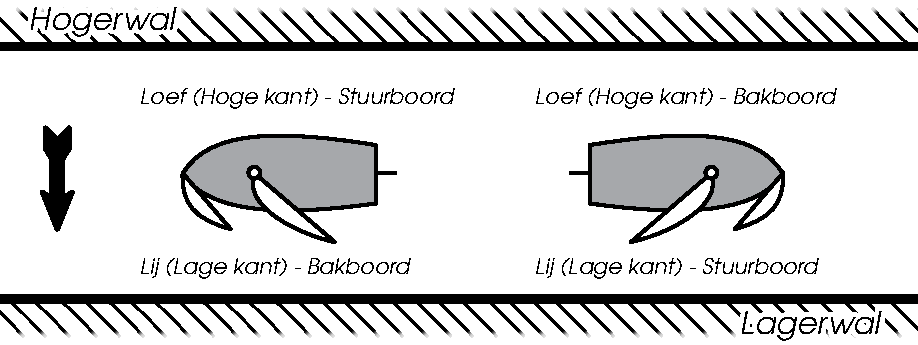
\includegraphics[width=0.9\textwidth]{Hoofdstukken/Onderdelen/pdf/wallen.pdf}
	\caption{Hoger- en Lagerwal}
	\centering
	\label{pic:hoog_laag}
\end{figure}

De hogerwal is de wal waar de wind vandaan komt. De lagerwal is de wal waar de wind naar toe waait. Al deze termen zijn te zien in figuur \ref{pic:hoog_laag}

\vfil\newpage

\subsection{Koersen}
Een koers vertelt iets over hoe je boot ligt ten opzichte van de wind. Alle koersen kun je zowel over bakboord, als stuurboord varen, behalve in de wind. Een overzicht van de koersen is te zien in figuur \ref{pic:koersen}. Wanneer je van koers verandert en naar de wind toe draait, loef je op. Wanneer je van de wind wegdraait heet dit afvallen. 

\begin{figure}[h]
	\centering
	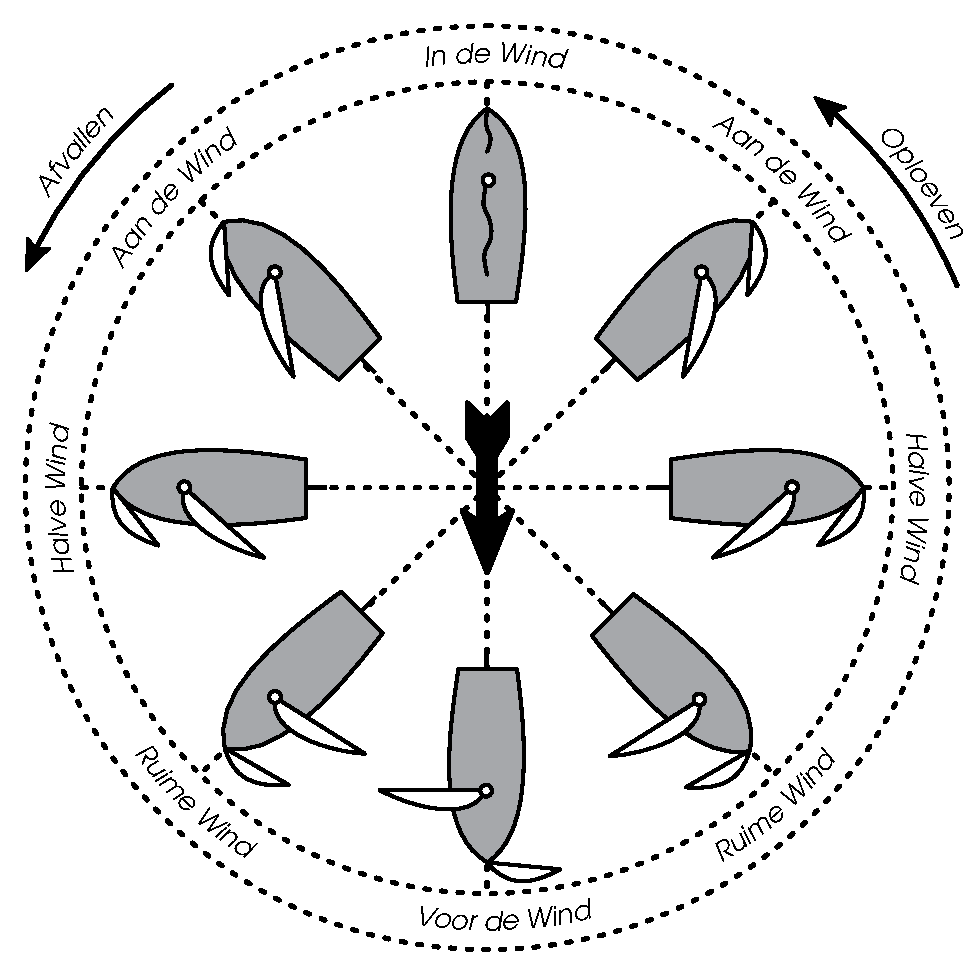
\includegraphics[width=0.9\textwidth]{Hoofdstukken/Onderdelen/pdf/koersen.pdf}
	\caption{Windkoersen}
	\label{pic:koersen}
\end{figure}



\subsection{Boven- en benedenwinds}
Op het water kan je vaak op twee manieren ergens langs varen: bovenwinds en benedenwinds. Bovenwinds houdt in dat je ergens langs vaart aan de kant waar de wind ernaartoe blaast, de hoge kant van het object. Benedenwinds is het tegenovergestelde: dit is de kant waar de wind van het object weg blaast en dus de lage kant van het object. Deze termen zijn te zien in figuur \ref{pic:boven_benedenwinds}.
\begin{figure}[h]
  \centering
  \begin{minipage}[b]{0.7\textwidth}
   \centering
    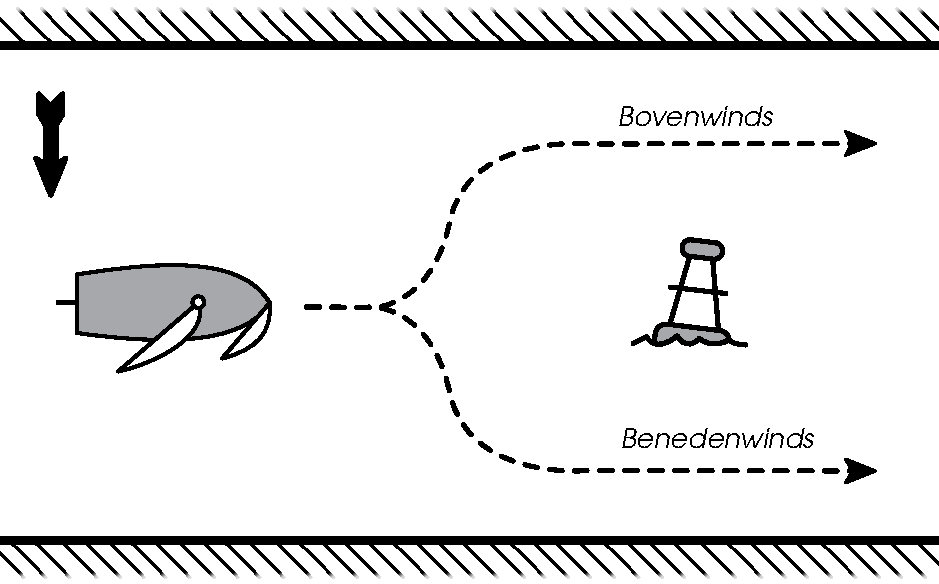
\includegraphics[width=0.9\textwidth]{Hoofdstukken/Onderdelen/pdf/boven_en_benedenwinds.pdf}
    \caption{Boven- en benedenwinds passeren van een boei}
    \centering
    \label{pic:boven_benedenwinds}
  \end{minipage}
  \hfill
  \begin{minipage}[b]{0.29\textwidth}
    \centering
    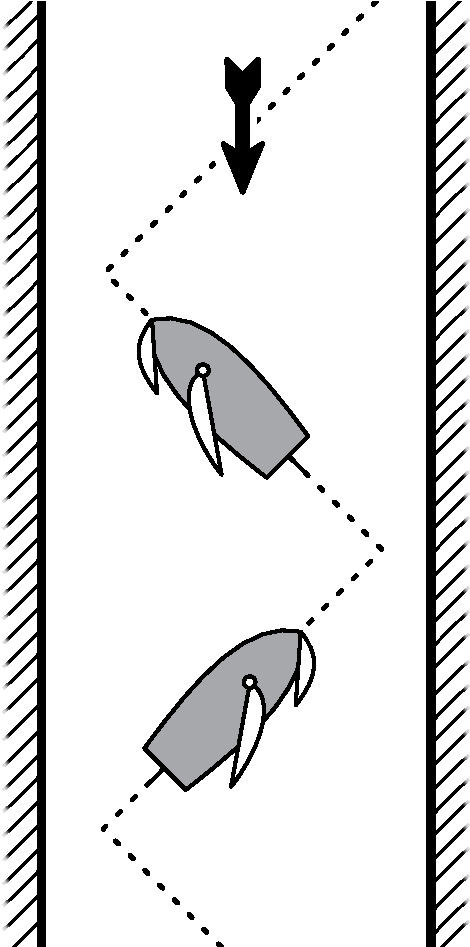
\includegraphics[width=0.7\textwidth]{Hoofdstukken/Onderdelen/pdf/opkruisen.pdf}
    \caption{Opkruisen}
    \label{pic:opkruisen}
  \end{minipage}
\end{figure}



Tip: De termen boven- en benedenwinds kunnen goed van pas komen bij een zeilwedstrijd. Hier wordt vaak aangegeven of je een boei boven- of benedenwinds moet ronden.

\newpage
\subsection{Overig}
Hiernaast dien je ook bekend te zijn met de onderstaande termen:

\begin{itemize}
    \item \textit{Overstag}: Je gaat hier van aan de wind over de ene boeg naar aan de wind over de andere boeg. Bijvoorbeeld: van aan de wind over bakboord naar aan de wind over stuurboord.
    \item \textit{Gijpen}: Je gaat hier van voor de wind over de ene boeg naar voor de wind over de andere boeg. Bijvoorbeeld: van voor de wind over bakboord naar voor de wind over stuurboord.
    \item \textit{Opkruisen of laveren}: Hierbij vaar je tegen de wind in door steeds aan de wind te varen en dan overstag te gaan. Een voorbeeld hiervan is te zien in figuur \ref{pic:opkruisen}
    \item \textit{Killen van het zeil}: Je laat dan expres een deel van je zeil minder wind vangen. Dit doe je door je zeil te vieren totdat alleen het achterlijk nog wind vangt.
    \item \textit{Opschieten}: Wanneer je een lijn opschiet, rol je deze netjes op. Ook wel bekend als opbossen.
    \item \textit{Beleggen}: Als je een kikker belegt, leg je de lijn via een bepaalde knoop op de kikker. Deze knoop zal in het hoofdstuk `Schiemannen' behandeld worden.
    \item \textit{Bak}: Wanneer je je fok bak doet, zet je deze aan de hoge kant in plaats van de lage kant.
    \item \textit{Deinzen}: Dit is wanneer je achteruit dobbert met de neus van je boot in de wind. 
\end{itemize}


\newpage

\section{Bootonderdelen}
In figuur \ref{pic:vlet_nummers} is een tekening van een lelievlet te zien met maar liefst 88 gelabelde onderdelen. De namen van de onderdelen staan in tabel \ref{table:vletwel}. Alle onderdelen, behalve die met grijze nummers, moet je kennen.

\begin{figure}[h!]
	\centering
	\makebox[\textwidth][c]{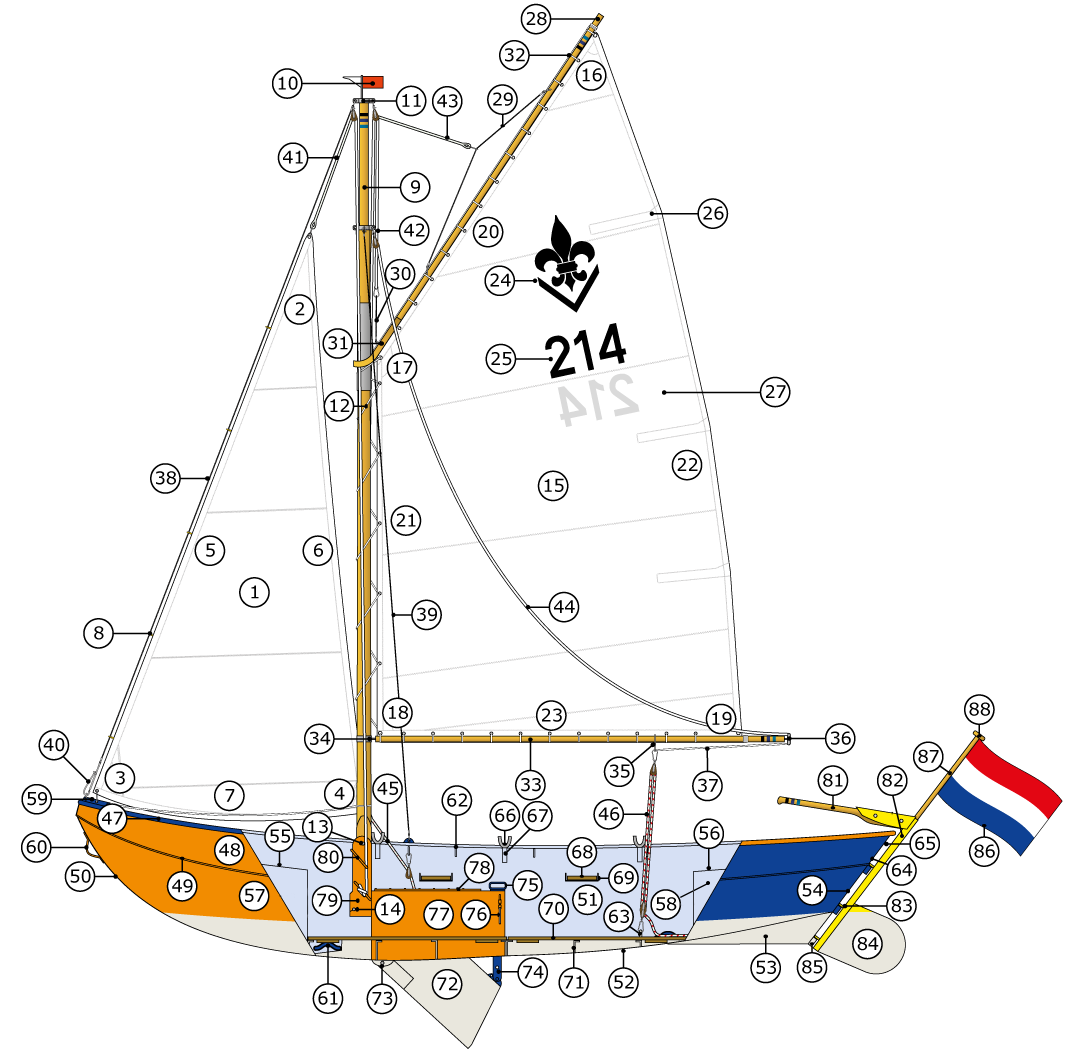
\includegraphics[width=1.2\textwidth]{Hoofdstukken/Onderdelen/png/lelievlet_onderdelen.png}}
	\caption{Tekening lelievlet met nummers \protect\footnotemark}
	\centering
	\label{pic:vlet_nummers}
\end{figure}

\footnotetext{\textit{Lelievlet\_onderdelen.png}, https://www.willibrordusgroep.nl/Images/upload/cwo/lelievlet\_onderdelen.png, Feb 2021.
}



\begin{table}[h!]
	\centering
	\caption{Vletonderdelen}
	
	\setlength\extrarowheight{5pt} %Add height to center text vertically
	\renewcommand{\arraystretch}{0.75} %Shrink total heigt to keep row same heigt
	\newcommand{\tabhead}[1]{\cellcolor{ocre}{\color[HTML]{FFFFFF}\sffamily \textbf{#1}}}
	\newcommand{\NIL}[1]{\cellcolor{not}{#1}}
	\label{table:vletwel}
	
	\begin{tabular}{|ll|ll|ll|ll|}
	\multicolumn{2}{|l|}{\tabhead{Fok}}       & \multicolumn{2}{l|}{\tabhead{Grootzeil}}   & \multicolumn{2}{l|}{\tabhead{Lopend want}} & \multicolumn{2}{l|}{\tabhead{Casco}}  \\
	\textbf{1}           & Fok               & \textbf{24}      & Zeilteken              & \textbf{45}        & Fokkeschoot          & \textbf{68}     & Doft               \\
	\textbf{2}           & Tophoek           & \textbf{25}      & Zeilnummer             & \textbf{46}        & Grootschoot          & \textbf{\NIL69} & Dofthouder         \\
	\textbf{3}           & Halshoek          & \textbf{26}      & Zeillat                & \multicolumn{2}{l|}{\tabhead{Casco}}      & \textbf{70}     & Vlonder/Denning    \\
	\textbf{4}           & Schoothoek        & \textbf{\NIL27}  & Baan                   & \textbf{47}        & Dolboord             & \textbf{71}     & Spant              \\
	\textbf{5}           & Voorlijk          & \multicolumn{2}{l|}{\tabhead{Gaffel}}     & \textbf{48}        & Boeisel              & \multicolumn{2}{l|}{\tabhead{Zwaard}} \\
	\textbf{\NIL6}       & Achterlijk        & \textbf{28}      & Gaffel                 & \textbf{49}        & Berghout             & \textbf{72}     & Zwaard             \\
	\textbf{\NIL7}       & Onderlijk         & \textbf{29}      & Spruit/gaffeldraad     & \textbf{50}        & Boeg                 & \textbf{73}     & Zwaardbout         \\
	\textbf{\NIL8}       & Leuver            & \textbf{\NIL 30} & Strop                  & \textbf{52}        & Vlak                 & \textbf{74}     & Zwaardloper        \\
	\multicolumn{2}{|l|}{\tabhead{Mast}}     & \textbf{31}      & Klauw                  & \textbf{53}        & Scheg                & \textbf{75}     & Zwaardgreep        \\
	\textbf{9}           & Mast              & \textbf{32}      & Marllijn               & \textbf{54}        & Spiegel              & \textbf{76}     & Zwaardpen          \\
	\textbf{10}          & Windvaantje       & \multicolumn{2}{l|}{\tabhead{Giek}}       & \textbf{55}        & Voordek              & \textbf{77}     & Zwaardkast         \\
	\textbf{\NIL11}      & Mastring          & \textbf{33}      & Giek                   & \textbf{56}        & Achterdek            & \textbf{78}     & Zwaardplaatje      \\
	\textbf{12}          & Rijglijn          & \textbf{34}      & Lummelbeslag           & \textbf{57}        & Kim                  & \textbf{79}     & Mastkoker          \\
	\textbf{13}          & Mastbout          & \textbf{35}      & Grootschootring        & \textbf{58}        & Luchtkast            & \textbf{80}     & Kikker             \\
	\textbf{14}          & Grendelbout       & \textbf{36}      & Wervel                 & \textbf{59}        & Hanenkam             & \multicolumn{2}{l|}{\tabhead{Roer}}   \\
	\multicolumn{2}{|l|}{\tabhead{Grootzeil}}& \textbf{37}      & Pettenlijntje          & \textbf{60}        & Sleepoog             & \textbf{81}     & Helmstok           \\
	\textbf{15}          & Grootzeil         & \multicolumn{2}{l|}{\tabhead{Staand want}}& \textbf{\NIL61}        & Hijsoog              & \textbf{82}     & Roerkoning         \\
	\textbf{16}          & Tophoek           & \textbf{38}      & Voorstag               & \textbf{\NIL62}    & Leioog               & \textbf{83}     & Roerhaak           \\
	\textbf{17}          & Klauwhoek         & \textbf{39}      & Zijstag                & \textbf{\NIL63}    & Grootschootoog       & \textbf{84}     & Roerblad           \\
	\textbf{18}          & Halshoek          & \textbf{\NIL 40} & Voorstagspanner        & \textbf{\NIL 64}   & Landvastoog          & \textbf{85}     & Vingerling         \\
	\textbf{19}          & Schoothoek        & \multicolumn{2}{l|}{\tabhead{Lopend want}}& \textbf{\NIL65}    & Wrikgat              & \multicolumn{2}{l|}{\tabhead{Vlag}}   \\
	\textbf{\NIL20}      & Bovenlijk         & \textbf{41}      & Fokkeval               & \textbf{66}        & Dol                  & \textbf{\NIL86}  & Vlag               \\
	\textbf{21}          & Voorlijk          & \textbf{42}      & Klauwval               & \textbf{67}        & Dolpot               & \textbf{\NIL87}  & Vlaggenstok        \\
	\textbf{22}          & Achterlijk        & \textbf{43}      & Piekeval               & \textbf{}          &                      & \textbf{\NIL88}  & Knop               \\
	\textbf{\NIL23}      & Onderlijk         & \textbf{44}      & Kraanlijn / dirk       & \textbf{}          &                      & \textbf{}       &                    \\ \hline
\end{tabular}
	
	\setlength\extrarowheight{0pt} %Reset
	\renewcommand{\arraystretch}{1} %Reset
	
\end{table}

\section{Conclusie}
Naast dat je nu bekend bent met de bootonderdelen uit tabel \ref{table:vletwel}, zijn dit al de zeiltermen uit de vorige paragrafen die je kent en begrijpt.
\begin{itemize}[label=]
\begin{multicols}{4}
	\item Bakboord
	\item Stuurboord
 	\item Loefzijde
	\item Lijzijde
    \item Hoge kant
    \item Lage kant
    \item Hogerwal
   	\item Lagerwal
    \item In de wind
    \item Aan de wind
    \item Halve wind
    \item Ruime wind
    \item Voor de wind
    \item Oploeven
    \item Afvallen
    \item Bovenwinds
    \item Benedenwinds
    \item Overstag
    \item Gijpen
    \item Opkruisen
    \item Laveren
    \item Killen van het zeil 
    \item Opschieten
    \item Beleggen
    \item Bak
    \item Deinzen

\end{multicols}
\end{itemize}

\header{3}
\chapter{Veiligheid, Weer \& Vaarproblematiek}
\section{Inleiding}
Wanneer je wil gaan zeilen is het belangrijk dat dit veilig gebeurt. Om voor deze veiligheid te zorgen zijn een aantal punten van groot belang. Hierbij kan je denken aan een reddingsvest, kennis van het weer, kennis van je boot maar ook dat van andere boten. Al deze punten worden in dit hoofdstuk behandeld.
\section{Reddingsvest}
Een reddingsvest is een belangrijk onderdeel van de veiligheid aan boord. Er zijn 5 situaties waar je een reddingsvest aan moet:
\begin{enumerate}
\begin{multicols}{2}
    \item Als je boots het zegt
    \item Als de staf het zegt
    \item Als de waterpolitie het zegt 
    \item Als je het zelf wilt 
    \item Wanneer je een regenjas, regenbroek of kaplaarzen aan hebt
\end{multicols}
\end{enumerate}
Daarnaast zijn er een aantal strenge eisen aan reddingsvesten. Een reddingsvest moet:
\begin{itemize}
    \item Je binnen 15 seconden op je rug draaien
    \item Je mond 7 cm boven de het water houden
    \item De tekst \textit{``Front''} aan de voorkant bevatten
    \item In het Nederlands gegevens over het drijfvermogen en maximaal gewicht van de drager bevatten
    \item De naam en het adres van de fabrikant bevatten
    \item Voorzien zijn van handvatten waar iemand mee uit het water getild kan worden
    \item Oranje of rood zijn.
\end{itemize}

\section{Omslaan}
Wanneer je boot is omgeslagen, \textbf{blijf je bij je boot}. Het is namelijk altijd gevaarlijker om te gaan zwemmen dan om bij je boot te blijven. Hier zijn een aantal redenen voor: ten eerste koel je veel minder snel af als je boven op je boot zit, of eraan hangt. Ook raak je zo minder vermoeid dan wanneer je zwemt. Daarnaast ben je makkelijker te vinden voor mensen die hulp willen bieden.
\section{Gedragsregels}
De belangrijkste en meest voorkomende gedragsregels zijn de volgende:
\begin{itemize}
    \item Houd de schippersgroet in ere
    \item Kom niet op iemands anders schip zonder toestemming
    \item Houd je schip en  omgeving schoon
    \item Het is gebruikelijk om zeilwedstrijden voorrang te geven / te vermijden
\end{itemize}
\subsection*{Schippersgroet}
Op het water is het een gewoonte om als schippers (roergangers) onderling naar elkaar te zwaaien. Dit staat bekend als ``de schippersgroet''. Niet alleen is het een vorm van beleefdheid, maar je weet hierdoor ook zeker dat de schipper van het andere schip jou gezien heeft. 

\section{Weersinvloeden}
Wanneer je gaat varen is het weer van groot belang. Samen met het soort boot, het soort vaarwater en de kennis en ervaring van je bemanning kan dit bepalen of het wel veilig is om het water op te gaan. Een van de belangrijkste weerfactoren is de windkracht.

De kracht van de wind wordt vaak uit gedrukt in de windschaal van Beaufort. De schaal bevat 13 verschillende niveaus. In vroegere tijden werd de wind bepaald aan de hand van de effecten op de omgeving. Tegenwoordig is de schaal van Beaufort gebaseerd op snelheden in km/u. In tabel \ref{tab:beafort} is een overzicht van de verschillende niveaus met bijbehorende snelheid en het effect op de omgeving. Met je CWO Kielboot III mag je maar varen tot en met windkracht 5.

\begin{table}[h]
	\centering
	\caption{Windschaal Beaufort}
	\label{tab:beafort}
	\begin{tabular}{C{2cm}|c|C{1.5cm}|p{7cm}}
		\textbf{Windkracht {[}Bft.{]}} & \textbf{Omschrijving} & \textbf{Snelheid {[}km/u{]}} & \textbf{Effect\protect\footnotemark[1] }                                  \\ \hline
		0                              & Stil                  & 0 - 1                        & Rook stijgt recht of bijna recht omhoog          \\
		1                              & Zwak                  & 1 - 5                        & Windrichting goed af te leiden uit rookpluimen   \\
		2                              & Zwak                  & 6 - 11                       & Wind merkbaar in gezicht                         \\
		3                              & Matig                 & 12 - 19                      & Stof waait op                                    \\
		4                              & Matig                 & 20 - 28                      & Haar in de war, kleding flappert                 \\
		5                              & Vrij krachtig         & 29 - 38                      & Gekuifde golven op meren en kanalen              \\
		6                              & Krachtig              & 39 - 49                      & Paraplu's met moeite vast te houden              \\
		7                              & Hard                  & 50 - 61                      & Lastig tegen de wind in te lopen of fietsen      \\
		8                              & Stormachtig           & 62 - 74                      & Voortbewegen zeer moeilijk                       \\
		9                              & Storm                 & 75 - 88                      & Dakpannen waaien weg, kinderen waaien om         \\
		10                            & Zware storm            & 89 - 102                     & \noindent\parbox[c]{\hsize}{Grote schade aan gebouwen, volwassenen waaien om} \\
		11                             & Zeer zware storm      & 102 - 117                    & Enorme schade aan bossen                         \\
		12                             & Orkaan                & \textgreater 117             & Verwoestingen                                   
	\end{tabular}
\end{table}

\subsection{Weersomslag}
Tijdens het varen is het verstandig om goed te letten op een weersomslag. Een weersomslag betekent dat het weer heel snel verandert. Het zou dus heel hard kunnen gaan waaien, regenen of zelfs stormen. Er zijn een aantal kenmerken die dit aan kunnen geven. 
\begin{itemize}
    \begin{multicols}{2}
    \item Snel opkomende bewolking of wind
    \item Bloemkoolwolken
    \item Stilte voor de storm
    \item Plotselinge wind draaiing
    \end{multicols}
\end{itemize}
Ook zijn er nog twee belangrijke termen die met wind draaiing te maken hebben. Dit zijn: ruimen en krimpen. Wanneer de wind ruimt, draait deze met de richting van de wijzers van de klok mee. Een krimpende wind is een wind draaiing die tegen de richting van de klok in gaat. Krimpende wind wordt vaak geassocieerd met het verslechten van het weer. Wanneer de wind dus sterk krimpt is het verstandig om het weer goed in de gaten te houden.
\footnotetext[1]{\textit{KNMI - Windschaal van Beaufort}, https://www.knmi.nl/kennis-en-datacentrum/uitleg/windschaal-van-beaufort, Okt 2022.
}

\newpage
\section{Vaarproblematiek andersoortige schepen}
\subsection{Dode hoek \hfill \textit{Figuur \ref{pic:dodehoek}}}
Net zoals in het verkeer bij vrachtauto's, kunnen grote schepen een dode hoek hebben. De dode hoek is het deel rondom het schip wat vanuit de stuurhut niet gezien kan worden. Sommige schepen hebben door hun vorm een dode hoek rondom het hele schip, niet alleen aan de voorkant. Als je bijvoorbeeld te dicht naast een schip vaart, kan de stuurman je mogelijk niet zien!

\subsection{Zuiging \hfill \textit{Figuur \ref{pic:zuiging}}}
Grote schepen hebben last van zuiging. De voorkant van het schip duwt het water weg en dit wordt aan de zij- en achterkant weer aangezogen. Kleine boten en zwemmers kunnen mee- of ondergezogen worden. Blijf dus uit deze gebieden weg.

  \begin{center}
  \begin{minipage}[b]{0.32\textwidth}
    \begin{figure}[H]
 		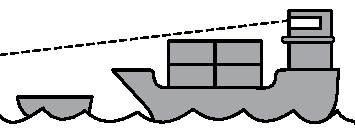
\includegraphics[width=\textwidth]{Hoofdstukken/Veiligheid/pdf/dode_hoek.pdf}
        \caption{Dode hoek}
        \label{pic:dodehoek}
    \end{figure}
  \end{minipage}
    \hspace{2cm}
  \begin{minipage}[b]{0.32\textwidth}
  \begin{figure}[H]
 		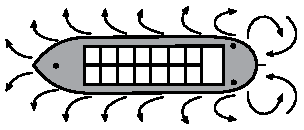
\includegraphics[width=\textwidth]{Hoofdstukken/Veiligheid/pdf/zuiging.pdf}
        \caption{Zuiging}
        \label{pic:zuiging}
    \end{figure}
  \end{minipage}
  \end{center}


\subsection{Diepgang  \hfill \textit{Figuur \ref{pic:diepgang}}}
Veel wateren hebben een vaargeul, dit is een dieper deel van het vaarwater. Soms is dit aangegeven met boeien of tonnen. Grote boten die zwaar beladen zijn kunnen soms alleen in dit deel van het water varen. Ze zullen misschien niet kunnen wijken voor je en jij zal daar rekening mee moeten houden.

\subsection{Verlijeren  \hfill \textit{Figuur \ref{pic:verlijeren}}}
Net als bij een zeilboot, kunnen ook grote motorschepen verlijeren. Als de wind van de zijkant komt, zal deze het schip opzij duwen. Om dit te corrigeren zal hij een beetje schuin gaan varen. Dit zorgt ervoor dat hij meer ruimte inneemt en minder wendbaar is. Geef deze schepen de ruimte. 

  \begin{center}
  \begin{minipage}[b]{0.30\textwidth}
    \begin{figure}[H]
        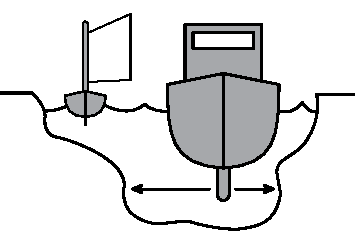
\includegraphics[width=\textwidth]{Hoofdstukken/Veiligheid/pdf/diepgang.pdf}
        \caption{Diepgang}
        \label{pic:diepgang}
    \end{figure}
  \end{minipage}
    \hspace{2cm}
  \begin{minipage}[b]{0.25\textwidth}
  \begin{figure}[H]
        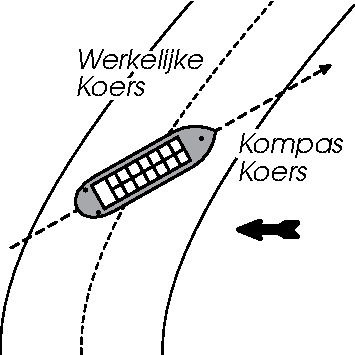
\includegraphics[width=\textwidth]{Hoofdstukken/Veiligheid/pdf/verlijeren.pdf}
        \caption{Verlijeren}
        \label{pic:verlijeren}
    \end{figure}
  \end{minipage}
  \end{center}


\section{Conclusie}
Je hebt in dit hoofdstuk geleerd wat belangrijk is om veilig te zeilen. Zo zijn er regels voor reddingsvesten, een gedragscode en is het slim om goed op het weer te letten - zowel voor als tijdens het varen. Als laatst is er nog gekeken naar vaarproblemen bij andere, voornamelijk grote, schepen.
\header{4}
\chapter{Bruggen \& Sluizen}
\section{Inleiding}
Bij langere tochten over het water zal je al snel te maken krijgen met bruggen en sluizen. In het BPR (Binnenvaart Politie Reglement) staan de regels voor het gebruiken hiervan gedefinieerd. In dit hoofdstuk worden deze regels uitgelegd om zo veilig een brug of sluis te kunnen passeren.

\section{Vaste bruggen}
Bruggen zijn te onderscheiden in twee soorten: vaste en beweegbare bruggen. Een vaste brug, zoals in figuur \ref{pic:brug:vast}, kan niet open. Bij een beweegbare brug is een of meerdere wegdelen van de brug beweegbaar om grotere schepen te laten passeren. 

De brug in figuur \ref{pic:brug:vast} heeft drie vaste brugopeningen. De linker opening heeft een rood bord met een witte streep. Dit betekent dat doorvaart verboden is. De middelste opening heeft een enkele gele ruit. Dit betekent dat doorvaart toegestaan is, maar dat tegenliggende vaart mogelijk is. De rechter opening heeft twee gele ruiten. Dit betekent dat doorvaart is toegestaan en tegenliggende vaart verboden is. Aan de achter kant van deze vaartopening zal dan ook een `doorvaart verboden' bord hangen. 

Als je de keuze hebt tussen een of twee gele ruiten, maak dan altijd gebruik van de optie met de twee ruiten. Deze is het veiligst omdat je geen tegenliggers kunt hebben.
\begin{figure}[ht!]
  \centering
    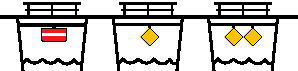
\includegraphics[width=0.7\textwidth]{Hoofdstukken/Bruggen/pdf/brug_vast.pdf}
    \caption{}
    \label{pic:brug:vast}
\end{figure}

\section{Beweegbare bruggen}
Naast vaste bruggen zijn er ook beweegbare bruggen. Deze bruggen hebben lichten in plaats van borden. Vaak heeft een beweegbare brug naast een beweegbare opening, ook een vaste opening. Deze openingen beschikken dan ook over borden of lichten.  

\newpage

% --- Beweegbaar verboden door te varen
\begin{figure}[H]
  \centering
  \begin{minipage}[b]{0.18\textwidth}
    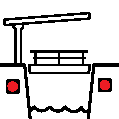
\includegraphics[width=\textwidth]{Hoofdstukken/Bruggen/pdf/brug_doorvaart_verboden.pdf}
    \caption{}
    \label{pic:brug:verboden}
  \end{minipage}
  \hfill
  \begin{minipage}[t]{0.75\textwidth}
  	\vspace{-2.5cm}
    Figuur \ref{pic:brug:verboden} betekent vrijwel hetzelfde als het rode bord uit figuur \ref{pic:brug:vast}. Doorvaart is verboden. Wanneer het echter de enige doorvaart is en je onder de gesloten brug past, mag je er wel door. Er kunnen dan ook tegenliggers aan komen.
  \end{minipage}
\end{figure}
% --- Beweegbaar doorvaart toegestaan, tegenliggende vaart mogelijk
\vspace{-0.75cm}
\begin{figure}[H]
	\centering
	\begin{minipage}[b]{0.18\textwidth}
		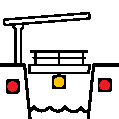
\includegraphics[width=\textwidth]{Hoofdstukken/Bruggen/pdf/brug_doorvaart_toegestaan.pdf}
		\caption{}
		\label{pic:brug:toegestaan}
	\end{minipage}
	\hfill
	\begin{minipage}[t]{0.75\textwidth}
	\vspace{-2.5cm}
	Figuur \ref{pic:brug:toegestaan} heeft de zelfde betekenis als een enkele gele ruit. De doorvaart is toegestaan, maar tegenliggende vaart is mogelijk. Wanneer je de optie hebt, kies dan voor de doorvaart met twee gele lichten. 
\end{minipage}
\end{figure}
% --- Beweegbaar doorvaart toegestaan, tegenliggende vaart niet mogelijk
\vspace{-0.75cm}
\begin{figure}[H]
\centering
\begin{minipage}[b]{0.18\textwidth}
	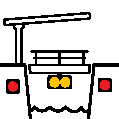
\includegraphics[width=\textwidth]{Hoofdstukken/Bruggen/pdf/brug_doorvaart_geen_tegenligger.pdf}
	\caption{}
	\label{pic:brug:toegestaan_tegenligger}
\end{minipage}
\hfill
\begin{minipage}[t]{0.75\textwidth}
	\vspace{-2.5cm}
	Figuur \ref{pic:brug:toegestaan_tegenligger} staat gelijk aan de twee gele ruiten. De doorvaart is toegestaan en tegenliggende vaart is niet mogelijk. Aan de andere kant van deze brug hangt een enkel rood licht of `verboden in te varen' bord.
\end{minipage}
\end{figure}
% --- Beweegbaar doorvaart aanstonds toegestaan
\vspace{-0.75cm}
\begin{figure}[H]
	\centering
	\begin{minipage}[b]{0.18\textwidth}
		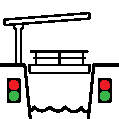
\includegraphics[width=\textwidth]{Hoofdstukken/Bruggen/pdf/brug_aanstonds_toegestaan.pdf}
		\caption{}
		\label{pic:brug:aanstonds}
	\end{minipage}
	\hfill
	\begin{minipage}[t]{0.75\textwidth}
		\vspace{-2.5cm}
		Wanneer je niet onder een brug past en deze beweegbaar is, kan hij voor je opengaan. Wanneer een brug bijna opengaat, gaan de lichten branden als in figuur \ref{pic:brug:aanstonds}. Doorvaart is nog verboden totdat alleen het groene licht brandt
	\end{minipage}
\end{figure}
% --- Beweegbaar doorvaart toegestaan
\vspace{-0.75cm}
\begin{figure}[H]
	\centering
	\begin{minipage}[b]{0.18\textwidth}
		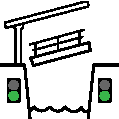
\includegraphics[width=\textwidth,]{Hoofdstukken/Bruggen/pdf/brug_toegestaan.pdf}
		\caption{}
		\label{pic:brug:vrij}
	\end{minipage}
	\hfill
	\begin{minipage}[t]{0.75\textwidth}
		\vspace{-2.5cm}
		Wanneer doorvaart door een beweegbare brug is toegestaan brandt er een enkel groen licht zoals in figuur \ref{pic:brug:vrij}. Het kan ook zijn dat wanneer de brug open is, je eerst een enkel rood licht krijgt. Dit betekent dat de tegenliggers eerst mogen. Hierna zul jij een groen licht krijgen.
	\end{minipage}
\end{figure}
% --- Beweegbaar doorvaart aanstonds verboden
\vspace{-0.75cm}
\begin{figure}[H]
	\centering
	\begin{minipage}[b]{0.18\textwidth}
		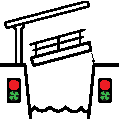
\includegraphics[width=\textwidth]{Hoofdstukken/Bruggen/pdf/brug_sluitend.pdf}
		\caption{}
		\label{pic:brug:sluitend}
	\end{minipage}
	\hfill
	\begin{minipage}[t]{0.75\textwidth}
		\vspace{-2.5cm}
		Wanneer een brug bijna gaat sluiten of aan het sluiten is, gaat er een groen knipperend en rood licht branden, zoals in figuur \ref{pic:brug:sluitend}. De doorvaart is nu verboden, tenzij je redelijkerwijs niet meer kan stoppen. Dit is dus vergelijkbaar met een oranje verkeerslicht. 
	\end{minipage}
\end{figure}
% --- Beweegbaar buiten gebruik
\vspace{-0.75cm}
\begin{figure}[H]
	\centering
	\begin{minipage}[b]{0.18\textwidth}
		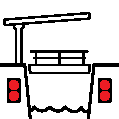
\includegraphics[width=\textwidth]{Hoofdstukken/Bruggen/pdf/brug_buiten_dienst.pdf}
		\caption{}
		\label{pic:brug:buiten}
	\end{minipage}
	\hfill
	\begin{minipage}[t]{0.75\textwidth}
		\vspace{-2.5cm}
		Als er een dubbel rood licht brandt (figuur \ref{pic:brug:buiten}), betekent het dat de brug buiten bediening is. De brugwachter kan dan bijvoorbeeld geen dienst hebben. Doorvaart is dan verboden. Wanneer er echter in het midden één of twee gele ruiten/lichten hangen gelden dezelfde regels als bij een enkel rood licht met gele ruit/licht.
	\end{minipage}
\end{figure}
% --- Beweegbaar gebied
\vspace{-0.75cm}
\begin{figure}[H]
	\centering
	\begin{minipage}[b]{0.18\textwidth}
		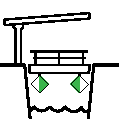
\includegraphics[width=\textwidth,]{Hoofdstukken/Bruggen/pdf/brug_aanbevolen_gebied.pdf}
		\caption{}
		\label{pic:brug:gebied}
	\end{minipage}
	\hfill
	\begin{minipage}[t]{0.75\textwidth}
		\vspace{-2.5cm}
		De ruiten in figuur \ref{pic:brug:gebied} geven iets aan over het aanbevolen vaargebied. Het is aanbevolen om binnen de groene ruiten te blijven varen. Dit kan te maken hebben met bijvoorbeeld een ondiepte of ander obstakel.
	\end{minipage}
\end{figure}
% --- Beweegbaar gebied verbod
\vspace{-0.75cm}
\begin{figure}[H]
\centering
\begin{minipage}[b]{0.18\textwidth}
	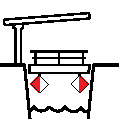
\includegraphics[width=\textwidth]{Hoofdstukken/Bruggen/pdf/brug_verboden_gebied.pdf}
	\caption{}
	\label{pic:brug:gebied_verbod}
\end{minipage}
\hfill
\begin{minipage}[t]{0.75\textwidth}
	\vspace{-2.5cm}
	Soms is het echter ook verboden om in bepaalde gebieden te varen. Dit wordt dan duidelijk gemaakt met de twee rode ruiten in figuur \ref{pic:brug:gebied_verbod}. Je moet dan tussen de rode ruiten in blijven en mag hier niet buiten varen.
\end{minipage}
\end{figure}

\section{Sluizen}
Een sluis wordt gebruikt om een boot te verplaatsen tussen twee wateren met een verschillende hoogte. Wanneer je een sluis in mag varen wordt net als bij bruggen bepaald door lichten.
Bij sluizen hebben de lichten vrijwel exact dezelfde betekenis als bij bruggen. Er zijn echter ook wat kleine verschillen. 

Vaak hangen er in een de sluis zelf ook lichten. Deze maken duidelijk wanneer je de sluis uit mag varen. Wanneer er een sluiswachter aanwezig is moet je goed naar zijn instructies luisteren. Hij geeft vaak aan waar je moet gaan liggen in de sluis. 

% --- Sluis verbod
\hfill
\begin{figure}[H]
	\centering
	\begin{minipage}[b]{0.18\textwidth}
		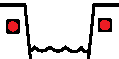
\includegraphics[width=\textwidth]{Hoofdstukken/Bruggen/pdf/sluis_verboden.pdf}
		\caption{}
		\label{pic:sluis:verbod}
	\end{minipage}
	\hfill
	\begin{minipage}[t]{0.75\textwidth}
		\vspace{-2cm}
		Figuur \ref{pic:sluis:verbod} betekent net als bij bruggen dat doorvaart verboden is. Ook als de deuren helemaal open zijn, moet je wachten tot de lichten groen worden. Als er boten in de sluis liggen, moeten deze er namelijk eerst uit.
	\end{minipage}
\end{figure}
% --- Sluis verbod aanstonds
\vspace{-0.35cm}
\begin{figure}[H]
	\centering
	\begin{minipage}[b]{0.18\textwidth}	
		
\includegraphics[width=\textwidth]{Hoofdstukken/Bruggen/pdf/sluis_aanstonds.pdf}
		\caption{}
		\label{pic:sluis:aanstonds}
	\end{minipage}
	\hfill
	\begin{minipage}[t]{0.75\textwidth}
		\vspace{-2cm}
		Wanneer de sluis bijna open gaat zullen de lichten aan gaan zoals in figuur \ref{pic:sluis:aanstonds}. Bij sommige sluizen is dit ook te zien als ze bijna gaan sluiten. Je mag er dan alleen nog in varen als je echt niet meer kan stoppen.
	\end{minipage}
\end{figure}
% --- Sluis toegestaan
\vspace{-0.35cm}
\begin{figure}[H]
	\centering
	\begin{minipage}[b]{0.18\textwidth}	
		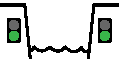
\includegraphics[width=\textwidth]{Hoofdstukken/Bruggen/pdf/sluis_toegestaan.pdf}
		\caption{}
		\label{pic:sluis:toegestaan}
	\end{minipage}
	\hfill
	\begin{minipage}[t]{0.75\textwidth}
		\vspace{-2cm}
		Wanneer je de sluis in mag varen, geeft de sluis een enkel groen licht. Dit is te zien in figuur \ref{pic:sluis:toegestaan}. Wanneer de lichten groen zijn zullen alle boten die eerst in de sluis zaten, deze verlaten hebben. 
	\end{minipage}
\end{figure}
% --- Sluis buiten bedrijf
\vspace{-0.35cm}
\begin{figure}[H]
	\centering
	\begin{minipage}[b]{0.18\textwidth}	
		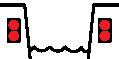
\includegraphics[width=\textwidth]{Hoofdstukken/Bruggen/pdf/sluis_buiten_dienst_dicht.pdf}
		\caption{}
		\label{pic:sluis:buiten}
	\end{minipage}
	\hfill
	\begin{minipage}[t]{0.75\textwidth}
		\vspace{-2cm}
		Een sluis kan net als een brug buiten bedrijf zijn. Dit wordt aangegeven met dubbele rode lichten uit figuur \ref{pic:sluis:buiten}. De deuren zullen in dit geval dicht zijn.
	\end{minipage}
\end{figure}
% --- Sluis buiten toegestaan
\vspace{-0.35cm}
\begin{figure}[H]
	\centering
	\begin{minipage}[b]{0.18\textwidth}	
		
\includegraphics[width=\textwidth]{Hoofdstukken/Bruggen/pdf/sluis_buiten_dienst_open.pdf}
		\caption{}
		\label{pic:sluis:buiten_toegestaan}
	\end{minipage}
	\hfill
	\begin{minipage}[t]{0.75\textwidth}
		\vspace{-2cm}
		Het kan ook voorkomen dat de sluis buiten bedrijf is, maar doorvaart is toegestaan. Beide deuren staan dan open en de sluis geeft een dubbel groen licht, zie figuur \ref{pic:sluis:buiten_toegestaan}
	\end{minipage}
\end{figure}

\paragraph{Brug en sluis combinatie}
Het komt wel eens voor dat er een sluis en brug direct naast elkaar geplaatst zijn. Let hierbij goed op de lichten. Het kan voorkomen dat je vrij lang voor de open brug moet wachten omdat de sluis eerst leeg moet varen. Wacht dus achter de brug, ook al pas je onder de brug door!

\section{Conclusie}
In dit hoofdstuk zijn alle lichten, tekens en regels voor bruggen en sluizen behandeld. Je weet nu wanneer het verboden en toegestaan is om een brug of sluis door te varen. Deze kennis is bijvoorbeeld heel erg van belang op een hike. Veel van de lichten hebben een logische betekenis en lijken soms zelfs een beetje op verkeerslichten. 

\header{5}
\chapter{Reglementen \& Voorrangsregels}
\section{Inleiding}
In dit hoofdstuk gaan we kijken naar de regels en wetten op het water. Op de meeste wateren waar jullie zullen varen wordt gebruik gemaakt van het Binnenvaart Politie Reglement, het BPR. Het BPR bevat alle regels over hoe je met elkaar om moet gaan op het water.

\section{Algemene reglementen}
Om het BPR goed te kunnen begrijpen, zullen we eerst een aantal algemene zaken bespreken. We beginnen met vier definities; motorschip, zeilschip, klein schip en groot schip. 

\begin{itemize}
    \item \textbf{Motorschip:} Een schip dat mechanische middelen gebruikt om zich voort te bewegen, een motor dus.
    \item \textbf{Zeilschip:} Een schip dat \textbf{alleen} zijn zeilen gebruikt om voort te bewegen. Hier onder valt ook een surfplank, maar niet een zeilboot met een motor aan.
    \item \textbf{Klein schip:} Alle schepen onder de 20 meter, met uitzondering van: passagiersschip \footnote{Draagt overdag een gele ruit achter op het schip om dit aan te duiden}, veerpont, visser, sleepboot
(alleen als deze grote schepen sleept), duwboot en duwbak. Deze uitzonderingen zijn altijd grote schepen. 
    \item \textbf{Groot schip:} Schepen groter dan 20 meter, inclusief de eerdergenoemde uitzonderingen 
\end{itemize}

\subsection{Goed zeemanschap}
Het goed zeemanschap is een hele belangrijke regel op het water. Deze regel houdt in dat de schipper bij het ontbreken van duidelijke regels \textbf{alle nodige voorzorgsmaatregelen} moet nemen om de veiligheid te garanderen, schade te voorkomen of de doorstroom op het water te versoepelen. Ook mag een schipper voor eigen veiligheid of die van anderen afwijken van het BPR.

\subsection{Andere reglementen}
Het BPR geldt niet op alle wateren. Het is verstandig om vooraf (als je op voor jou onbekende wateren gaat varen) uit te zoeken welke regels er gelden. Dit kan bijvoorbeeld in de ANWB Wateralmanak. In deel 1 staan alle regels en wetten die gelden in Nederland en België. 

\newpage
\section{Voorrangsregels}
Voorrangssituaties zijn te verdelen in drie types: kruisende koersen, tegengestelde koeren en oplopende koersen. Deze drie zijn te zien in figuur \ref{pic:voorrangkoers}. Welke van deze situaties je vaart bepaalt met welke regels je te maken hebt. 
\begin{figure}[H]
    \centering
    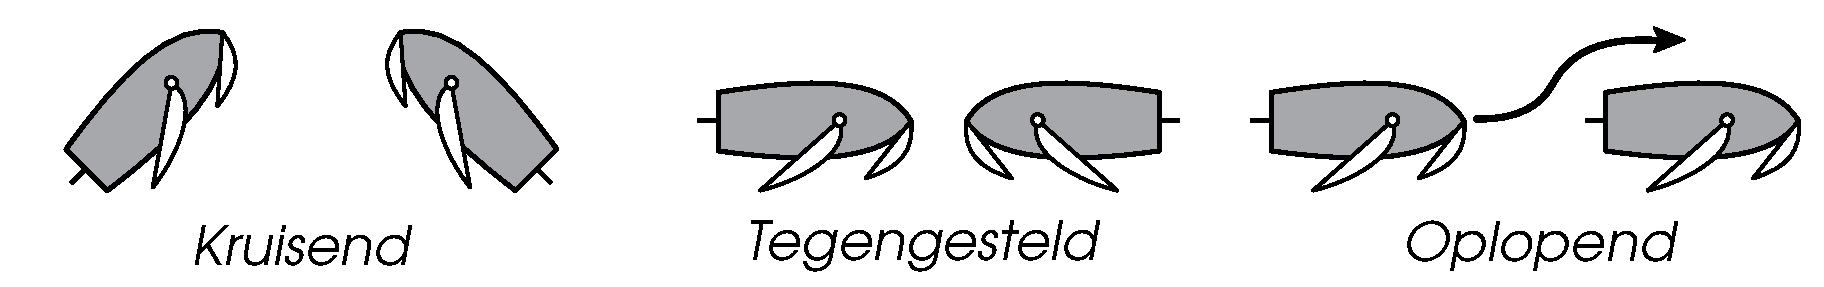
\includegraphics[width=0.8\textwidth]{Hoofdstukken/Reglementen/pdf/voorrangskoersen.pdf}
    \caption{Voorrangskoersen}
    \centering
    \label{pic:voorrangkoers}
\end{figure}
De voorrangsregels hebben ook een volgorde. Na het bepalen van welke koers je vaart, kijk je altijd eerst naar de bovenste regel die hierbij hoort. Als deze regel niet van toepassing is, ga je pas door naar de volgende. Dit doe je net zo lang tot er een regel is die toe te passen is op jouw situatie.


\paragraph{Kruisende koersen}
\vspace{-0.7cm}
\begin{figure}[H]
	\centering
	\begin{minipage}[t]{0.70\textwidth}
		\textbf{1.} Het schip wat aan de stuurboordswal vaart heeft voorrang.\\
		\textit{Zeilschip A vaart aan de stuurboordswal en heeft voorrang op B}
	\end{minipage}
	\hfill
	\begin{minipage}[t]{0.20\textwidth}
		\raisebox{-0.5\height}{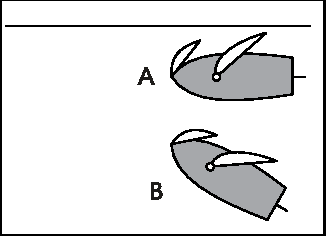
\includegraphics[width=\textwidth]{Hoofdstukken/Reglementen/pdf/kruis_stuurboordswal.pdf}}
		\label{pic:kr1}
	\end{minipage}
	\hfill
\end{figure}

\vspace{-0.7cm}

\begin{figure}[H]
	\centering
	\begin{minipage}[t]{0.70\textwidth}
		\textbf{2.} Grote schepen hebben voorrang op kleine schepen.\\
		\textit{Het grote motorschip A heeft voorrang op het kleine motorschip B}
	\end{minipage}
	\hfill
	\begin{minipage}[t]{0.20\textwidth}
		\raisebox{-0.5\height}{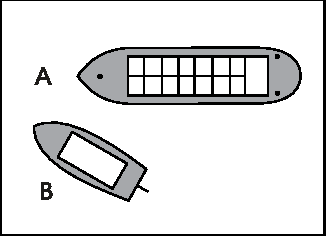
\includegraphics[width=\textwidth]{Hoofdstukken/Reglementen/pdf/kruis_groot_klein.pdf}}	
		\label{pic:kr2}
	\end{minipage}
	\hfill
\end{figure}

\vspace{-0.7cm}
\begin{figure}[H]
	\centering
	\begin{minipage}[t]{0.72\textwidth}
		\textbf{3.} Schepen op het hoofdvaarwater gaan voor op het nevenvaarwater.\\
		\textit{Motorschip A op het hoofddvaarwater heeft voorrang op motorschip B}
	\end{minipage}
	\hfill
	\begin{minipage}[t]{0.20\textwidth}
		\raisebox{-0.5\height}{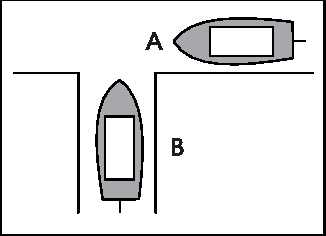
\includegraphics[width=\textwidth]{Hoofdstukken/Reglementen/pdf/kruis_hoofd_neven.pdf}}	
		\label{pic:kr3}
	\end{minipage}
	\hfill
\end{figure}

\vspace{-0.7cm}
\begin{figure}[H]
	\centering
	\begin{minipage}[t]{0.70\textwidth}
		\textbf{4.} Een zeilschip gaat voor een roeiboot gaat voor een motorschip.\\
		\textit{Zeilschip A heeft voorrang op roeiboot B en motorschip C\\
			Roeiboot B heeft voorrang op motorschip C}
	\end{minipage}
	\hfill
	\begin{minipage}[t]{0.20\textwidth}
		\raisebox{-0.65\height}{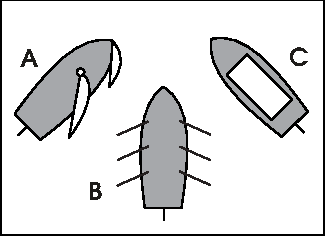
\includegraphics[width=\textwidth]{Hoofdstukken/Reglementen/pdf/kruis_zsm.pdf}}	
		\label{pic:kr4}
	\end{minipage}
	\hfill
\end{figure}

\vspace{-0.7cm}
\begin{figure}[H]
	\centering
	\begin{minipage}[t]{0.70\textwidth}
		\textbf{5.} Motor- en roeiboten onderling: Het schip van rechts gaat voor.\\
		\textit{Motorschip A op rechts heeft voorrang op motorschip B}
	\end{minipage}
	\hfill
	\begin{minipage}[t]{0.20\textwidth}
		\raisebox{-0.65\height}{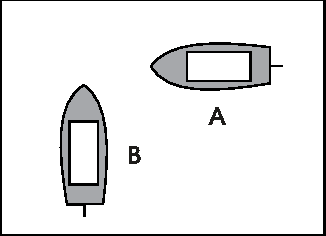
\includegraphics[width=\textwidth]{Hoofdstukken/Reglementen/pdf/kruis_motor_onderling.pdf}}	
		\label{pic:kr5}
	\end{minipage}
	\hfill
\end{figure}

\vspace{-0.7cm}

\textbf{6.} Bij zeilschepen onderling zijn de volgende twee regels van belang:
\vspace{-0.5cm}
\begin{figure}[H]
	\centering
	\hspace{0.02\textwidth}
	\begin{minipage}[t]{0.70\textwidth}
		\textbf{6.1}. Een zeilschip met zeilen over bakboord heeft voorrang.\\
		\textit{Zeilschip B (met zijn zeilen over bakboord) heeft voorrang op \\zeilschip A (met zijn zeilen over stuurboord)}
	\end{minipage}
	\hfill
	\begin{minipage}[t]{0.20\textwidth}
		\raisebox{-0.6\height}{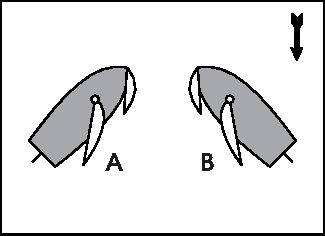
\includegraphics[width=\textwidth]{Hoofdstukken/Reglementen/pdf/kruis_zeilboot_onderling_bakboord.pdf}}	
		\label{pic:kr41}
	\end{minipage}
	\hfill
\end{figure}

\vspace{-0.7cm}
\begin{figure}[H]
	\centering
	\hspace{0.02\textwidth}
	\begin{minipage}[t]{0.70\textwidth}
		\textbf{6.2.} Een zeilschip aan loef wijkt voor een zeilschip aan lij.\\
		\textit{Zeilschip A ligt aan loef van zeilschip B en verleent dus voorrang}
	\end{minipage}
	\hfill
	\begin{minipage}[t]{0.20\textwidth}
		\raisebox{-0.55\height}{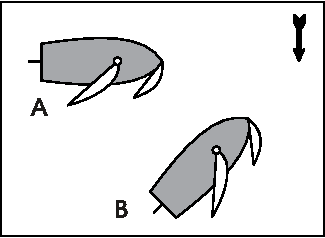
\includegraphics[width=\textwidth]{Hoofdstukken/Reglementen/pdf/kruis_zeilboot_onderling_loef_lij.pdf}}	
		\label{pic:kr42}
	\end{minipage}
	\hfill
\end{figure}

\paragraph{Tegengestelde koersen}
\vspace{-0.2cm}
\begin{figure}[H]
	\centering
	\begin{minipage}[t]{0.70\textwidth}
		\textbf{1.} Het schip wat aan de stuurboordswal vaart heeft voorrang.\\
		\textit{Zeilschip B vaart aan de stuurboordswal en heeft voorrang op A}
	\end{minipage}
	\hfill
	\begin{minipage}[t]{0.25\textwidth}
		\raisebox{-0.55\height}{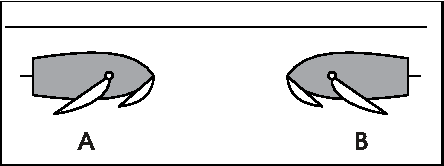
\includegraphics[width=\textwidth]{Hoofdstukken/Reglementen/pdf/tegen_stuurboord.pdf}}
		\label{pic:tg1}
	\end{minipage}
	\hfill
\end{figure}
\vspace{-0.7cm}

\begin{figure}[H]
	\centering
	\begin{minipage}[t]{0.70\textwidth}
		\textbf{2.} Grote schepen hebben voorrang op kleine schepen.\\
		\textit{Het grote motorschip B heeft voorrang op het kleine motorschip A}
	\end{minipage}
	\hfill
	\begin{minipage}[t]{0.25\textwidth}
		\raisebox{-0.55\height}{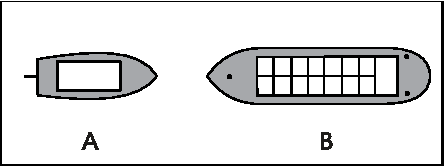
\includegraphics[width=\textwidth]{Hoofdstukken/Reglementen/pdf/tegen_groot_klein.pdf}}
		\label{pic:tg2}
	\end{minipage}
	\hfill
\end{figure}
\vspace{-0.7cm}

\begin{figure}[H]
	\centering
	\begin{minipage}[t]{0.70\textwidth}
		\textbf{3.} Een zeilschip gaat voor een roeiboot gaat voor een motorschip.\\
		\textit{Zeilschip A heeft voorrang op roeiboot B \\
			Zeilschip C heeft voorrang op motorschip D \\
			Roeiboot E heeft voorrang op motorschip F}
	\end{minipage}
	\hfill
	\begin{minipage}[t]{0.25\textwidth}
		\raisebox{-0.75\height}{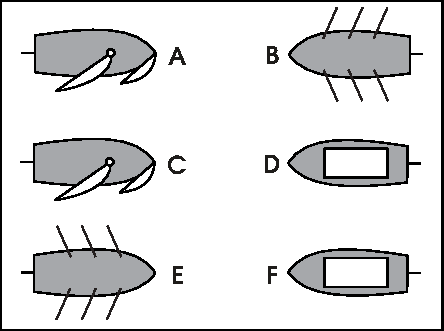
\includegraphics[width=\textwidth]{Hoofdstukken/Reglementen/pdf/tegen_zsm.pdf}}
		\label{pic:tg3a}
	\end{minipage}
	\hfill
\end{figure}
\vspace{-0.7cm}

\begin{figure}[H]
	\centering
	\begin{minipage}[t]{0.70\textwidth}
		\textbf{4.} Zeilschepen onderling: Een zeilschip met zeilen over bakboord heeft voorrang.\\
		\textit{Zeilschip B (met zijn zeilen over bakboord) heeft voorrang op A}
	\end{minipage}
	\hfill
	\begin{minipage}[t]{0.25\textwidth}
		\raisebox{-0.75\height}{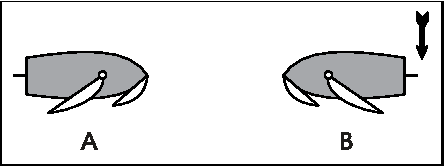
\includegraphics[width=\textwidth]{Hoofdstukken/Reglementen/pdf/tegen_zeilboot_onderling.pdf}}	
		\label{pic:tg4}
	\end{minipage}
	\hfill
\end{figure}
\vspace{-0.7cm}

\begin{figure}[H]
	\centering
	\begin{minipage}[t]{0.70\textwidth}
		\textbf{5.} Roei- of motorschepen onderling: Beide wijken naar stuurboord.\\
		\textit{Beide motorschepen wijken naar stuurboord}
	\end{minipage}
	\hfill
	\begin{minipage}[t]{0.25\textwidth}
		\raisebox{-0.55\height}{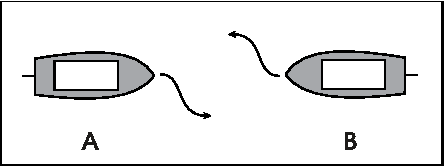
\includegraphics[width=\textwidth]{Hoofdstukken/Reglementen/pdf/tegen_motor_spier_onderling.pdf}}	
		\label{pic:tg5}
	\end{minipage}
	\hfill
\end{figure}

\paragraph{Oplopen}
Oplopen is \textit{enkel} toegestaan wanneer dit gedaan kan worden zonder gevaar voor andere schepen. Oplopen wordt voornamelijk langs bakboord gedaan. Het is echter ook toegestaan, wanneer de situatie hier om vraagt, om langs stuurboord op te lopen.

\begin{figure}[H]
	\centering
	\begin{minipage}[t]{0.70\textwidth}
		Zeilschepen onderling lopen elkaar op via de loefzijde. Hierdoor neem je de wind uit de zeilen van het opgelopen schip en gaat het oplopen sneller. Tijdens het oplopen mag medewerking verlangd worden van het opgelopen schip.
	\end{minipage}
	\hfill
	\begin{minipage}[t]{0.25\textwidth}
		\raisebox{-0.8\height}{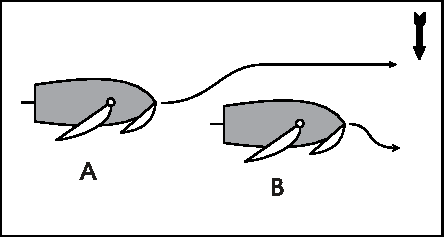
\includegraphics[width=\textwidth]{Hoofdstukken/Reglementen/pdf/oplopen.pdf}}
		\label{pic:op}
	\end{minipage}
	\hfill
\end{figure}

\newpage
\subsection{Voorrangsregels op een rij}
Om de voorrangsregels makkelijk te kunnen onthouden staan ze hieronder samengevat:\\[0.1cm]
Bij \textbf{kruisende koersen} kijk je naar de volgende regels:
\vspace*{-0.15cm}
\begin{enumerate}
	\item Het stuurboordswal varende schip gaat voor
	\item Grote schepen gaan voor op kleine schepen
	\item Hoofdwater gaat voor nevenwater
	\item Zeilschip gaat voor roeiboot gaat voor motorschip
	\item Roei- of motorschepen onderling: het schip van rechts gaat voor
	\item Zeilschepen onderling: 
	\stepcounter{enumi}
	\begin{enumerate}
		\item [1.]Zeilen over bakboord gaat voor
		\item [2.]Loef wijkt voor lij
	\end{enumerate}
\end{enumerate}

Bij \textbf{tegengestelde koersen} kijk je naar de volgende regels:
\vspace*{-0.15cm}
\begin{enumerate}
	\item Het stuurboordswal varende schip gaat voor
	\item Grote schepen gaan voor op kleine schepen
	\item Zeilschip gaat voor roeiboot gaat voor motorschip
	\item Zeilschepen onderling: zeilen over bakboord gaat voor
	\item Roei- of motorschepen onderling: beiden wijken naar stuurboord
\end{enumerate}

Bij \textbf{oplopende koersen}, wijkt de oploper uit. Het opgelopen schip kan indien nodig uitwijken.

\subsection{Toevoegingen}
\begin{figure}[H]
	\centering
	\begin{minipage}[t]{0.65\textwidth}
		Wanneer je vaarwater oversteekt, heb je geen voorrang. Andere schepen moeten hun koers en snelheid niet of nauwelijks hoeven aan te passen voor jouw manoeuvre. \\
		
		
		De regel `Stuurboordswal gaat voor' gaat over de stuurboordszijde van het \textbf{vaarwater}, niet over de echte wal. Boot A en B in figuur \ref{pic:SBwal} varen dus beide aan stuurboordswal, ondanks dat zij niet aan een fysieke wal varen.
	\end{minipage}
	\hfill
	\begin{minipage}[t]{0.30\textwidth}
		\raisebox{-0.9\height}{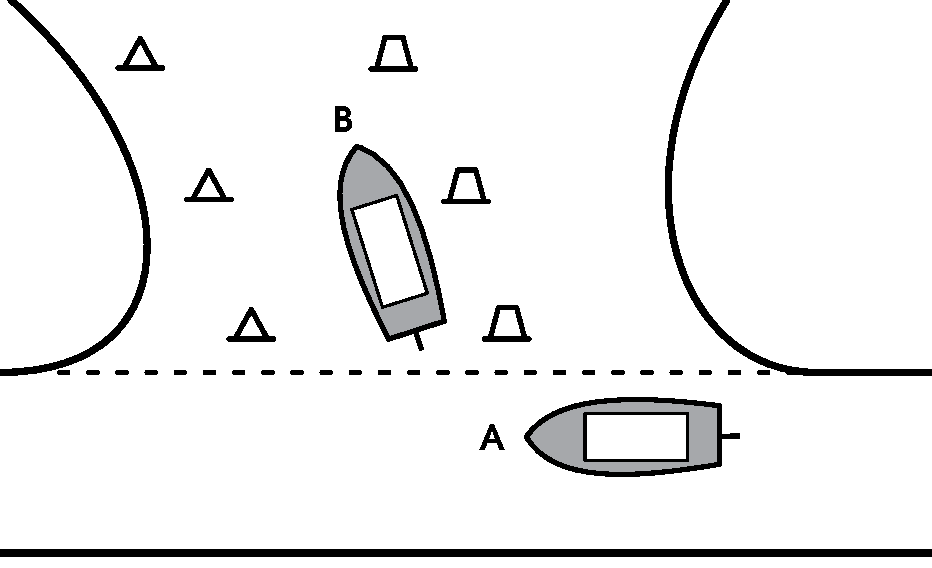
\includegraphics[width=\textwidth]{Hoofdstukken/Reglementen/pdf/sb_wal.pdf}}
		\caption{}
		\label{pic:SBwal}
	\end{minipage}
\end{figure}


\section{Conclusie}
Na het lezen van dit hoofdstuk heb je verstand van de voorrangsregels op het water. Een van de belangrijkste is het goed zeemanschap, wat inhoudt dat je alles doet om een gevaarlijke situatie of aanvaring te voorkomen. Daarnaast ken je de verschillende voorrangssituaties en volgorde en weet je hoe je de regels moet toepassen. 
\header{7}
\chapter{Schiemannen}
\section{Inleiding}
In dit hoofdstuk worden de knopen geleerd die belangrijk zijn tijdens het varen. Je moet de knopen kunnen maken en begrijpen wanneer en waarom je ze gebruikt. Ook word je geacht een aantal verschillende soorten touwen te kunnen onderscheiden en hun voordelen te begrijpen.

\section{Touwsoorten, toepassing en terminologie}

\paragraph{Gevlochten en geslagen}
Een touw kan opgebouwd worden op twee manieren: geslagen en gevlochten. Beide touwen hebben voor- en nadelen waardoor er niet één superieur is aan de ander. Waar een geslagen touw vaak goedkoper is, loopt een gevlochten touw soepeler door blokken. Om deze redenen zie je vaak beide touwen op een boot.

\paragraph{Schavielen}
Wanneer een touw constant op dezelfde plek ergens tegen aan schuurt, is deze aan het schavielen. Dit kan bijvoorbeeld gebeuren wanneer je afgemeerd bent en een landvast tegen de kade schuurt. Een dweil tussen je landvast en de kade kan dit verhelpen.

\paragraph{Touwsoorten}
Tegenwoordig wordt aan boord voornamelijk touw van kunstvezel gebruikt waar dit vroeger veel natuurvezeltouw was. Om de sterktes en zwaktes van een kunstvezel touw beter te begrijpen is in tabel \ref{table:touwwerk} een vergelijking gemaakt tussen de twee touwsoorten.

\begin{table}[h]
	\centering
	\caption{Verschil in touwsoorten}
	\label{table:touwwerk}
	\begin{tabular}{c|c}
		\textbf{Natuurvezel} & \textbf{Kunstvezel} \\ \hline
		Rek en krimpen bij nat en droog worden & Geen rek \\ \hline
		Geringe breeksterkte & Hoge breeksterkte \\ \hline
		Bestand tegen UV-straling & Matig bestand tegen UV-straling \\ \hline
		Slijtvast bij schavielen & Gevoelig voor schavielen
	\end{tabular}
\end{table}

\paragraph{Toepassingen soorten touw}
Verschillende situaties vragen om verschillende touwsoorten. Hieronder is een kort overzicht van het meest geschikte touw voor verschillende situaties.
\begin{itemize}
	\item \textbf{Schoten:} Schoten moeten soepel door de blokken lopen voor gebruiksgemak. Dit maakt een gevlochten touw erg geschikt.
	\item \textbf{Ankerlijn en landvasten:} Voor landvasten en ankerlijnen is een kleine mate van rek gunstig. Deze vangen namelijk de klappen van plotselinge bewegingen op.
	\item \textbf{Vallen:} Voor een val is een touw zonder rek belangrijk. Dit maakt het hijsen makkelijker en voorkomt dat deze zeilen later `inzakken'.
\end{itemize}


\section{De knopen}
\subsection{Halve steek \hfill \hspace{2 cm} \textit{Figuur \ref{pic:halve_steek}} } 
Een halve steek leg je wanneer je een lijn vast wil leggen waar weinig kracht op komt. De halve steek is de basis voor veel knopen en steken.
\subsection{Slipsteek \hfill \textit{Figuur \ref{pic:slip_steek}}}
De slipsteek kan alleen gebruikt worden in situaties waar weinig kracht op de lijn komt. Het voordeel van een slipsteek is dat hij snel los te maken is.
\subsection{Achtknoop \hfill \textit{Figuur \ref{pic:achtknoop}}}
Een achtknoop wordt gebruikt om een verdikking in een lijn te maken. Hiermee voorkom je bijvoorbeeld dat een lijn door een blok schiet. 

\begin{figure}[h]
  \centering
  \begin{minipage}[b]{0.32\textwidth}
  \centering
    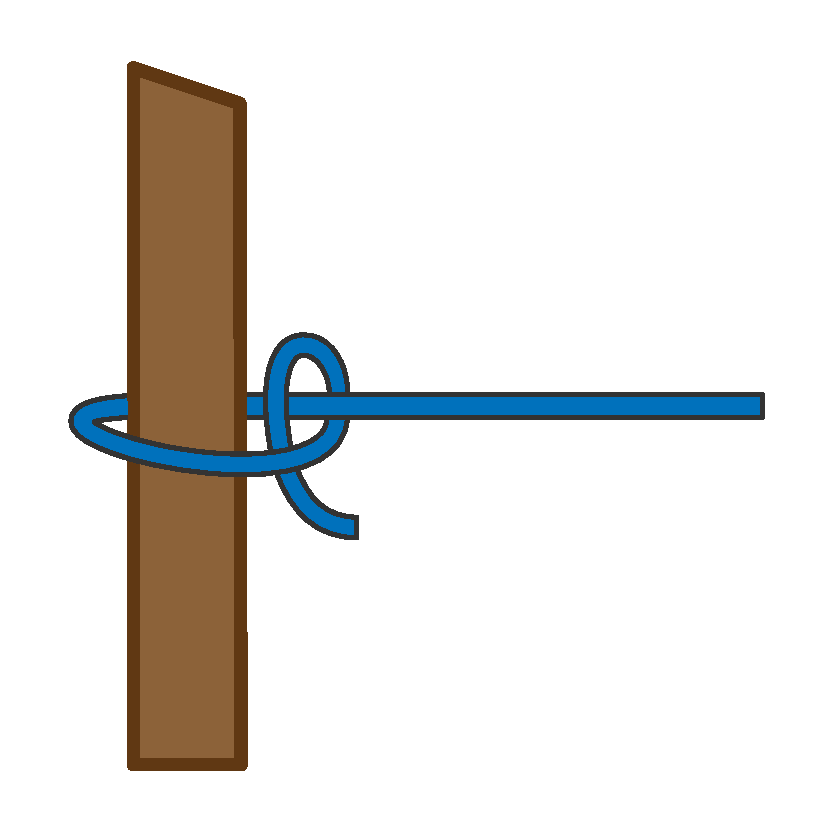
\includegraphics[height=4cm]{Hoofdstukken/Schiemannen/pdf/halve_steek.pdf}
    \caption{Halve steek}
    \label{pic:halve_steek}
  \end{minipage}
  \hfill
  \begin{minipage}[b]{0.32\textwidth}
    \centering
    \includegraphics[height=4cm]{Hoofdstukken/Schiemannen/pdf/slip_steek.pdf}
    \caption{Slipsteek}
    \label{pic:slip_steek}
    \end{minipage}
  \hfill
  \begin{minipage}[b]{0.32\textwidth}
    \centering
    \includegraphics[height=4cm]{Hoofdstukken/Schiemannen/pdf/achtknoop.pdf}
    \caption{Achtknoop}
    \label{pic:achtknoop}
  \end{minipage}
\end{figure}

\subsection{Platte knoop \hfill \textit{Figuur \ref{pic:platte_knoop}}}
Deze knoop is geschikt voor het verbinden van twee uiteinde van een lijn van gelijke dikte. Deze knoop is niet geschikt voor situaties waar veel kracht op de lijn komt te staan. Hiervoor is een schootsteek beter geschikt.
\subsection{Schootsteek \hfill \textit{Figuur \ref{pic:schoot_steek}}}
Een schootsteek is geschikt om twee lijnen van ongelijke dikte aan elkaar te maken. De knoop is ook geschikt voor lijnen van gelijke dikte en kan veel kracht aan. Bij lijnen van ongelijke dikte wordt met de dikke lijn de `lus' (blauw) gelegd, dit maakt de knoop makkelijker. Wanneer er extreem veel kracht op de knoop komt, kan deze dubbel gelegd worden. In dit geval wordt de `lus' een extra keer omwikkeld. 
 
\begin{figure}[h]
  \centering
  \begin{minipage}[b]{0.32\textwidth}
  \centering
    \includegraphics[height=4cm]{Hoofdstukken/Schiemannen/pdf/platteknoop.pdf}
    \caption{Platte knoop}
    \label{pic:platte_knoop}
  \end{minipage}
  \hfill
  \begin{minipage}[b]{0.64\textwidth}
    \centering
    \includegraphics[height=4cm]{Hoofdstukken/Schiemannen/pdf/schootsteek.pdf}
    \hspace*{1cm}
    \includegraphics[height=4cm]{Hoofdstukken/Schiemannen/pdf/dubbele_schootsteek.pdf}
    \caption{Schootsteek enkel en dubbel}
    \label{pic:schoot_steek}
    \end{minipage}
  \hfill
\end{figure}
\subsection{Mastworp \hfill \textit{Figuur \ref{pic:mastworp}}}
Deze knoop wordt veel gebruikt in pionieren en om je boot aan te leggen. De knoop trekt zich zelf strakker naar mate er meer kracht op komt. Daarnaast kun je een slipsteek op een mastworp leggen. Dit voorkomt dat de mastworp los kan schieten als er veel aan getrokken wordt.
\subsection{Paalsteek \hfill \textit{Figuur \ref{pic:paal_steek}}} 
De paalsteek is bedoeld om een niet slippende lus in een lijn te leggen. De lus is erg sterk, maar kan wel gemakkelijk weer losgehaald worden.
\subsection{Een tros opschieten \hfill \textit{Figuur \ref{pic:opschieten}}}
Een tros opschieten is een manier om een lijn op te bergen zonder dat deze in de knoop raakt. Tijdens het opschieten maak je een aantal gelijke lussen. Aan het einde wikkel je de rest van de lijn om de lussen en leg je een knoop als in het figuur. Opschieten staat ook wel bekend als opbossen.
\begin{figure}[h]
  \centering
  \begin{minipage}[b]{0.32\textwidth}
  \centering
    \includegraphics[height=4cm]{Hoofdstukken/Schiemannen/pdf/mastworp.pdf}
    \caption{Mastworp}
    \label{pic:mastworp}
  \end{minipage}
  \hfill
  \begin{minipage}[b]{0.32\textwidth}
    \centering
    \includegraphics[height=4cm]{Hoofdstukken/Schiemannen/pdf/paalsteek.pdf}
    \caption{Paalsteek}
    \label{pic:paal_steek}
    \end{minipage}
  \hfill
   \begin{minipage}[b]{0.32\textwidth}
    \centering
    \includegraphics[height=4cm]{Hoofdstukken/Schiemannen/pdf/opbossen.pdf}
    \caption{Opschieten}
    \label{pic:opschieten}
    \end{minipage}
\end{figure}


\subsection{Dubbele halve steek \hfill \textit{Figuur \ref{pic:dub_halve_steek} \& \ref{pic:dub_slip_halve_steek}}}
Een dubbele halve steek is geschikt om lijnen strak aan een oog vast te maken. Dit is bijvoorbeeld handig als aan wilt leggen met een meerpen. Je wikkelt eerst de lijn tweemaal om een oog en legt er vervolgens twee halve steken in. Dit maakt een mastworp. Je kan de eerste halve steek ook vervangen door een slipsteek om hem makkelijker los te maken. Dit is te zien in figuur \ref{pic:dub_slip_halve_steek}.


\begin{figure}[h]
	\centering
	\begin{minipage}[b]{0.49\textwidth}
		\centering
		\includegraphics[height=4cm]{Hoofdstukken/Schiemannen/pdf/dubble_halve_steek.pdf}
		\caption{Dubbele halve steek}
		\label{pic:dub_halve_steek}
	\end{minipage}
	\hfill
	\begin{minipage}[b]{0.49\textwidth}
		\centering
		\includegraphics[height=4cm]{Hoofdstukken/Schiemannen/pdf/dubble_halve_steek_slippend.pdf}
		\caption{Slippende dubbele halve steek}
		\label{pic:dub_slip_halve_steek}
	\end{minipage}
	\hfill
\end{figure}
\newpage
\subsection{Een kikker beleggen \hfill \textit{Figuur \ref{pic:kikker1}, \ref{pic:kikker2} \& \ref{pic:kikker3}}}
Wanneer je een kikker belegt, leg je een lijn vast op een kikker. Dit is nodig voor bijvoorbeeld het hijsen van het zeil. Belangrijk bij het beleggen van een kikker in een boot is dat je de ''eindlus'' aan de bovenzijde van de kikker legt. Anders kan deze er afvallen en de kikker losraken. Daarnaast moet je het lusje zo draaien dat het uiteinde weer in de richting van het vorige achtje gaat.
\begin{figure}[h]
  \centering
  \begin{minipage}[b]{0.32\textwidth}
  \centering
    \includegraphics[width=\textwidth]{Hoofdstukken/Schiemannen/pdf/kikker1.pdf}
    \caption{Kikker 8'tjes}
    \label{pic:kikker1}
  \end{minipage}
  \hfill
  \begin{minipage}[b]{0.32\textwidth}
    \centering
    \includegraphics[width=\textwidth]{Hoofdstukken/Schiemannen/pdf/kikker2.pdf}
    \caption{Kikker eind lus}
    \label{pic:kikker2}
    \end{minipage}
  \hfill
   \begin{minipage}[b]{0.32\textwidth}
    \centering
    \includegraphics[width=\textwidth]{Hoofdstukken/Schiemannen/pdf/kikker3.pdf}
    \caption{Kikker afknopen}
    \label{pic:kikker3}
    \end{minipage}
\end{figure}
\section{Conclusie}
Na het lezen van dit hoofdstuk en het oefenen met de knopen, snap je het nut en toepassing van de verschillende knopen. Ook kan je alle knopen zonder voorbeeld leggen. Een instructeur heeft dit in de onderstaande tabel afgetekend.
\vspace{2cm}
\begin{table}[H]
\centering
\caption{Aftekenen knopen}
\label{my-label}
\begin{tabular}{|l|l|l|}
\hline
\textbf{Knoop of Handeling}  & \textbf{Paraaf} & \textbf{Paraaf} \\ \hline
\textit{Halve Steek}         &                 &                 \\ \hline
\textit{Slipsteek}          &                 &                 \\ \hline
\textit{Achtknoop}           &                 &                 \\ \hline
\textit{Platte Knoop}        &                 &                 \\ \hline
\textit{Schootsteek}        &                 &                 \\ \hline
\textit{Dubbele schootsteek}        &                 &                 \\ \hline
\textit{Mastworp}            &                 &                 \\ \hline
\textit{Paalsteek}           &                 &                 \\ \hline
\textit{Dubbele halve steek} &                 &                 \\ \hline
\textit{Slippende dubbele halve steek} &                 &                 \\ \hline
\textit{Tros opschieten}     &                 &                 \\ \hline
\textit{Kikker beleggen}     &                 &                 \\ \hline
\end{tabular}
\end{table}
\header{7}
\chapter{Krachten op het schip}
\section{Inleiding}
In voorbereiding op het leren van een aantal zeilmanoeuvres is het belangrijk om de krachten op het schip goed te snappen. In dit hoofdstuk gaan we onder andere kijken naar hoe krachten weergegeven kunnen worden en de verschillende effecten van deze krachten. 
\section{Krachten weergeven}
Een kracht wordt weergegeven met een pijl. De richting van de pijl geeft de richting van de kracht weer en de lengte geeft de grootte van de kracht weer. In figuur \ref{pic:kracht} is een voorbeeld te zien.

De wind wordt meestal met één pijl aangegeven. In werkelijkheid komt de wind meer als een vlak op je af. Het zijn als het ware heel veel pijlen met dezelfde richting naast elkaar. Dit is te zien in figuur \ref{pic:wind_pijl}.

Tot slot is er nog het draaipunt. Wanneer er een kracht op een voorwerp met draaipunt gezet wordt, draait deze om het draaipunt. Bij een boot zit het draaipunt ongeveer bij de mast. In figuur \ref{pic:draaipunt} is hier een voorbeeld van gegeven. Je zou de tekening een beetje met een wip kunnen vergelijken.
\begin{figure}[h]
  \centering
  \begin{minipage}[b]{0.32\textwidth}
  \centering
    \includegraphics[width=0.8\textwidth]{../Hoofdstukken/Krachten/pdf/krachten.pdf}
    \caption{Krachten}
    \label{pic:kracht}
  \end{minipage}
  \hfill
  \begin{minipage}[b]{0.32\textwidth}
    \centering
    \includegraphics[width=0.8\textwidth]{Hoofdstukken/Krachten/pdf/wind.pdf}
    \caption{Wind pijlen}
    \label{pic:wind_pijl}
    \end{minipage}
  \hfill
  \begin{minipage}[b]{0.32\textwidth}
    \centering
    \includegraphics[width=0.8\textwidth]{Hoofdstukken/Krachten/pdf/draaipunt.pdf}
    \caption{Draaipunt}
    \label{pic:draaipunt}
  \end{minipage}
\end{figure}
\section{Effecten van de fok en het grootzeil}
Het grootzeil en de fok hebben allebei een ander effect op de boot. Omdat de fok voor het draaipunt zit, zorgt deze voor afvallen. Dit is te zien in figuur \ref{pic:effect_fok}.

Het grootzeil doet het tegenovergestelde omdat deze achter het draaipunt zit. Hierdoor zal de boot gaan oploeven. Dit effect is weergegeven in figuur \ref{pic:effect_grootzeil}.
\begin{figure}[ht]
  \centering
  \begin{minipage}[b]{0.49\textwidth}
  \centering
    \includegraphics[width=0.8\textwidth]{../Hoofdstukken/Krachten/pdf/effect_fok.pdf}
    \caption{Effect van de fok}
    \label{pic:effect_fok}
  \end{minipage}
  \hfill
  \begin{minipage}[b]{0.49\textwidth}
    \centering
    \includegraphics[width=0.8\textwidth]{../Hoofdstukken/Krachten/pdf/effect_grootzeil.pdf}
    \caption{Effect van het grootzeil}
    \label{pic:effect_grootzeil}
    \end{minipage}
\end{figure}
\section{Correcte zeilstand}
We beginnen door te kijken naar wanneer het grootzeil goed staat. Een voorbeeld van een zeil wat goed staat is te zien in figuur \ref{pic:zeil_goed}. De windpijlen stormen mooi, dicht langs het zeil. Het zeil vervormt niet door de wind en staat mooi bol.

Wanneer je het zeil echter te strak aan trekt, zie je in figuur \ref{pic:zeil_strak} dat de wind pijlen aan de buitenkant van het zeil "loslaten". De wind wil liever rechtdoor dan dicht langs het zeil. Hierdoor ontstaan er in dit stukje wervelingen. Door deze wervelingen gaat het achterlijk van je zeil klapperen. Je zeil staat niet meer goed en hierdoor ga je langzamer zeilen.    
\begin{figure}[H]
  \centering
  \begin{minipage}[b]{0.32\textwidth}
  \centering
    \includegraphics[width=0.85\textwidth]{Hoofdstukken/Krachten/pdf/zeil_goed.pdf}
    \caption{Zeil goed}
    \label{pic:zeil_goed}
  \end{minipage}
  \hfill
  \begin{minipage}[b]{0.32\textwidth}
    \centering
    \includegraphics[width=0.85\textwidth]{../Hoofdstukken/Krachten/pdf/zeil_strak.pdf}
    \caption{Zeil te strak}
    \label{pic:zeil_strak}
    \end{minipage}
  \hfill
  \begin{minipage}[b]{0.32\textwidth}
    \centering
    \includegraphics[width=0.85\textwidth]{Hoofdstukken/Krachten/pdf/zeil_los.pdf}
    \caption{Zeil te los}
    \label{pic:zeil_los}
  \end{minipage}
\end{figure}
Een andere manier waar op je zeil verkeerd kan staan is als hij te los is. Dit is afgebeeld in figuur \ref{pic:zeil_los}. Het zeil zit nu als het ware in de weg van de wind. De windpijlen botsen bij het voorlijk van je zeil met het zeil. Hierdoor ontstaat er een tegen bolling dicht bij je mast. Dit remt je ook af. 

Een goede manier om je zeil te stellen, is om hem net zo lang te laten vieren, totdat je een kleine tegenbolling ziet in het voorlijk. Dan trek je het zeil weer een klein beetje aan. Op deze manier benut je de wind maximaal. Door dit regelmatig te doen weet je zeker dat je optimaal zeilt. 
\section{Effect van de helling}
De helling van je boot (oftewel, hoe schuin je vaart) heeft ook effect op het gedrag van de boot. Met name op de loef- en lijgierigheid. Uit zichzelf is de boot loefgierig. Dit houdt in dat de boot vanzelf de wind in draait als er niets gebeurt. 

Door de boot te laten hellen naar de lijkant, kan je dit effect versterken. Hoe meer mensen er bijvoorbeeld aan de lijkant in de boot zitten, hoe sneller de boot oploeft. Het tegenovergestelde geldt voor de loefkant. Als je naar deze kant helt, wil de boot uit zichzelf afvallen. 
\section{Conclusie}
In dit hoofdstuk zijn de verschillende krachten op het schip behandeld. Je snapt nu wanneer een zeil goed en fout staat en hoe je je zeil makkelijk goed kan zetten. Daarnaast snap je welke krachten er op het schip zijn, wat ze doen en hoe je deze in je voordeel kunt gebruiken.  

\makeatletter\@addtoreset{chapter}{part}
\makeatother 

\part{Oefenvragen}
\label{part:oefen}
\thispagestyle{empty}
\makeatletter\@openrightfalse
\makeatother
\setcounter{chapter}{0}
\usechapterimagefalse
\chapter{Bootonderdelen \& Zeiltermen}
\vspace{-120px}

\question{1}{Hoe heet de bovenste rand van het casco?}
\answerTextFour{Boeisel}{Berghout}{Dolboord}{Kim}
\question{2}{Hoe heet het opstaande randje op het voordek waar de voorstag aan vast zit?}
\answerTextFour{Sleepoog}{Hanekam}{Boeisel}{Voorstaghouder}
\question{3}{Tegen de wind in zeilen door steeds overstag te gaan heet:}
\answerTextFour{Kruisrak}{Opkruisen}{Laveren}{Alle bovenstaande antwoorden zijn goed}

\question{4}{Hoe heet de hoek van het zeil aangegeven in het plaatje?}
\vspace*{-1cm}
\answerTextPicture{Tophoek}{Halshoek}{Klauwhoek}{Schoothoek}{Hoofdstukken/Oefenvragen/pdf/tophoek.pdf}


\question{5}{Welk onderdeel wijst de pijl aan?}
\answerTextPicture{Roerkoningen}{Roerhaakgaten}{Roerpennen}{Vingerlingen}{Hoofdstukken/Oefenvragen/pdf/vingerlingen.pdf}

\question{6}{Welke stelling is waar?}
\answerTextPicture{I is de hogerwal en III is de lage kant}{II is de hogerwal en III is lagerwal}{IV is de lagerwal en II is de hogerwal}{II is de lage kant en III is de hoge kant}{Hoofdstukken/Oefenvragen/pdf/wallen.pdf}

\question{7}{Met welk lijntje hijs je de fok?}
\answerTextFour{Fokkeval}{Fokkelijn}{Fokkeschoot}{Grootschoot}
\newpage
\question{8}{Op welke afbeelding vaart de boot ruime wind?}
\answerPicture{Hoofdstukken/Oefenvragen/pdf/aan_de_wind.pdf}{Hoofdstukken/Oefenvragen/pdf/voor_de_wind.pdf}{Hoofdstukken/Oefenvragen/pdf/ruime_wind.pdf}{Hoofdstukken/Oefenvragen/pdf/halve_wind.pdf}


\question{9}{Welke stelling is waar?}%boven en benede winds
\answerTextPicture{De boot rondt de boei bovenwinds over bakboord}{De boot rondt de boei bovenwinds over stuurboord}{De boot rondt de boei benedenwinds over bakboord}{De boot rondt de boei benedenwinds over stuurboord.}{Hoofdstukken/Oefenvragen/pdf/bovenwinds_over_stuurboord_ronden.pdf}

\question{10}{Wat gebeurt er met je boot als je gaat oploeven?}%boven en benede winds
\answerTextFour{Je boot draait van de wind af}{Je  draait door de wind heen}{Je draait naar de wind toe}{Je boot ligt in de wind}



\chapter{Veiligheid, Weer \& Vaarproblematiek}
\vspace{-120px}

\question{1}{Wat is geen eis aan een reddingsvest?}
\answerTextFour{Oranje of rood van kleur zijn}{Naam en adres van de fabrikant bevatten}{Handvatten hebben waarmee iemand uit het water getild kan worden}{Binnen 7 seconden op je rug draaien}

\question{2}{Wat is een gedragsregel op het water?}
\answerTextFour{Houd de schippersgroet in ere}{Kom niet op andermans schip zonder toestemming}{Houd je schip en omgeving schoon}{A, B en C zijn alledrie juist}

\question{3}{Wanneer de wind plots snel draait kan dit wijzen op:}
\answerTextFour{Een weersomslag}{Opkomende bewolking}{Groter wordende golven}{A, B en C zijn alledrie juist}

\question{4}{Waarom moet je bij je boot blijven als die is omgeslagen}
\answerTextFour{Omdat naar de kant zwemmen gevaarlijk is}{Omdat je de boot niet alleen mag laten}{Om je de boot anders kwijt kunt raken}{Omdat dat gezelliger is}

\question{5}{Waar moet je op letten als je een groot schip ziet verlijeren?}
\answerTextFour{Dat deze minder goed kan sturen}{Dat deze meer ruimte in beslag neemt}{Dat de boot plots kan opschuiven}{Dat er meer zuiging is}

\question{6}{Waar is de zuiging het ergst bij een groot schip?}
\answerTextFour{De voorkant}{De voor- en achterkant}{De zijkant}{De zij- en achterkant}

\question{7}{Wat gebeurt er wanneer de wind krimpt?}
\answerTextFour{Het gaat zachter waaien}{De wind draait tegen de richting van de klok in}{De wind draait met de richting van de klok mee}{De windvlagen worden zachter}

\question{8}{De dode hoek van een groot schip is}
\answerTextFour{Waar de schipper niets kan zien}{De hoek waar de meeste zuiging is}{De hoek die het schip met het water maakt}{De achterkant van het schip}

\chapter{Bruggen \& Sluizen}
\vspace{-120px}
\question{1}{Bij welke brug is doorvaart toegestaan en is tegenliggende vaart verboden?}


\begin{figure}[H]
	\centering
	\begin{minipage}[b]{0.23\textwidth}
		\includegraphics[width=\textwidth]{Hoofdstukken/Bruggen/pdf/brug_doorvaart_toegestaan.pdf}
		\centering
		A
	\end{minipage}
	\hfill
	\begin{minipage}[b]{0.23\textwidth}
		\includegraphics[width=\textwidth]{Hoofdstukken/Bruggen/pdf/brug_doorvaart_geen_tegenligger.pdf}
		\centering
		B
	\end{minipage}
	\hfill
	\begin{minipage}[b]{0.23\textwidth}
		\includegraphics[width=\textwidth]{Hoofdstukken/Bruggen/pdf/brug_doorvaart_verboden.pdf}
		\centering
		C
	\end{minipage}
	\hfill
	\begin{minipage}[b]{0.23\textwidth}
		\includegraphics[width=\textwidth]{Hoofdstukken/Bruggen/pdf/brug_aanstonds_toegestaan.pdf}
		\centering
		D
	\end{minipage}
\end{figure}


\question{2}{Welke brug gaat bijna open?}

\begin{figure}[H]
	\centering
	\begin{minipage}[b]{0.23\textwidth}
		\includegraphics[width=\textwidth]{Hoofdstukken/Bruggen/pdf/brug_aanstonds_toegestaan.pdf}
		\centering
		A
	\end{minipage}
	\hfill
	\begin{minipage}[b]{0.23\textwidth}
		\includegraphics[width=\textwidth]{Hoofdstukken/Bruggen/pdf/brug_sluitend.pdf}
		\centering
		B
	\end{minipage}
	\hfill
	\begin{minipage}[b]{0.23\textwidth}
		\includegraphics[width=\textwidth]{Hoofdstukken/Bruggen/pdf/brug_toegestaan.pdf}
		\centering
		C
	\end{minipage}
	\hfill
	\begin{minipage}[b]{0.23\textwidth}
		\includegraphics[width=\textwidth]{Hoofdstukken/Bruggen/pdf/brug_doorvaart_toegestaan.pdf}
		\centering
		D
	\end{minipage}
\end{figure}

\question{3}{Wat betekenen de groene borden op deze burg?}
\begin{figure}[H]	
	\vspace{-10px}
	\begin{minipage}[]{0.70\textwidth}
		\begin{enumerate}[topsep=0pt, label=\Alph*.]
			\item Brug buiten bediening
			\item Het gebied tussen de borden is het aangeraden vaargebied
			\item Doorvaart toegestaan
			\item Doorvaart toegestaan, tegenliggers mogelijk
		\end{enumerate}
	\end{minipage}
	\begin{minipage}[]{0.29\textwidth}
		\begin{figure}[H]
			\includegraphics[width=0.80\textwidth,right]{Hoofdstukken/Bruggen/pdf/brug_aanbevolen_gebied.pdf}
		\end{figure}
	\end{minipage}
	\vspace{-10px}
\end{figure}

\question{4}{Wat betekent een enkele gele ruit?}
\answerTextFour{Doorvaart verboden}{Doorvaart toegestaan, tegenliggers mogelijk}{Doorvaart toegestaan, tegenliggers niet mogelijk}{Brug buiten bediening}

\question{5}{De brug gaat al naar beneden. Mag je er nog onder door varen?}
\begin{figure}[H]	
	\vspace{-10px}
	\begin{minipage}[]{0.70\textwidth}
		\begin{enumerate}[topsep=0pt, label=\Alph*.]
			\item Ja, het groene licht brandt nog
			\item Ja, zolang het nog past
			\item Nee, \textit{tenzij} je niet meer kan stoppen
			\item Nee, je mag nooit onder een sluitende brug door varen
		\end{enumerate}
	\end{minipage}
	\begin{minipage}[]{0.29\textwidth}
		\begin{figure}[H]
			\includegraphics[width=0.80\textwidth,right]{Hoofdstukken/Bruggen/pdf/brug_sluitend.pdf}
		\end{figure}
	\end{minipage}
	\vspace{-10px}
\end{figure}

\chapter{Reglementen \& Voorrangsregels}
\vspace{-120px}
\section*{Wie heeft er voorrang? Denk ook goed na waarom en vul de letter in!}
\begin{table}[h!]
\centering
\begin{tabular}{l|l|l|l|l|l|l|l|l|l|l|l|l|l|l}
\textbf{1} & \textbf{2} & \textbf{3} & \textbf{4} & \textbf{5} & \textbf{6} & \textbf{7} & \textbf{8} & \textbf{9} & \textbf{10} & \textbf{11} & \textbf{12} & \textbf{13} & \textbf{14} & \textbf{15} \\ \hline
 \hspace{0.5 cm} & \hspace{0.5 cm}  & \hspace{0.5 cm} & \hspace{0.5 cm} & \hspace{0.5 cm} & \hspace{0.5 cm} & \hspace{0.5 cm} & \hspace{0.5 cm} & \hspace{0.5 cm} & \hspace{0.5 cm} & \hspace{0.5 cm} & \hspace{0.5 cm} & \hspace{0.5 cm} & \hspace{0.5 cm}
\end{tabular}
\end{table}
\begin{figure}[h!]
    \centering
    \includegraphics[width=\textwidth]{Hoofdstukken/Oefenvragen/pdf/regelementen_1.pdf}
\end{figure}

\newpage
\begin{figure}[h!]
    \centering
    \includegraphics[width=\textwidth]{Hoofdstukken/Oefenvragen/pdf/regelementen_2.pdf}
\end{figure}
Bij sommige van de vorige situaties is een extra vraag. Het vraagnummer van de onderstaande vragen geeft aan naar welk figuur je moet kijken.\vspace{2cm}

\question{5}{Op welke volgorde mogen de boten verder varen?}
\answerTextFour{A-B-C}{C-B-A}{C-A-B}{B-C-A}

\question{9}{Welke koersen varen de schepen ten opzichte van elkaar?}
\answerTextFour{Kruisende koers}{Voorbijlopende koers}{Oplopende koers}{Tegengestelde koers}

\question{10}{Welke stelling is waar?}
\answerTextFour{B heeft voorrang want hij heeft zijn zeilen over bakboord}{A heeft voorrang, je kan namelijk niet zien over welke boeg zijn zeilen staan}{A heeft voorrang, hij vaart lij}{B moet uitwijken. A is stuurloos, er ontbreken regels dus goed zeemanschap geldt}

\question{12}{Wie heeft er voorrang en waarom?}
\answerTextFour{A, want zeil gaat voor spier gaat voor motor}{A, want B steekt een vaarwater over}{B, want hij vaart stuurboordwal}{B, want hij is aan het manoeuvreren}

\question{13}{Wie heeft er voorrang en waarom?}
\answerTextFour{A, want zeil gaat voor spier gaat voor motor}{B, want A steekt een vaarwater over}{B, want hij vaart stuurboordwal}{B, want A komt van links}
\chapter{Schiemannen}
\vspace{-120px}
\question{1}{Met welke knoop maak je twee touwen van ongelijke dikte aan elkaar vast?}
\answerTextFour{Schootsteek}{Paalsteek}{Constrictor}{Platte knoop}

\question{2}{Welke knoop zie je in de afbeelding hiernaast?}
	\vspace{-20px}
\begin{figure}[H]	

	\begin{minipage}[]{0.70\textwidth}
		\begin{enumerate}[topsep=0pt, label=\Alph*.]
			\item Een achtknoop
			\item Een platte knoop
			\item Een halve steek
			\item Een schootsteek
		\end{enumerate}
	\end{minipage}
	\begin{minipage}[]{0.29\textwidth}
		\begin{figure}[H]
			\includegraphics[width=0.80\textwidth,right]{Hoofdstukken/Schiemannen/pdf/platteknoop.pdf}
		\end{figure}
	\end{minipage}
	\vspace{-20px}
\end{figure}


\question{3}{Welke knoop leg je op een mastworp als iets voor lange tijd vast moet blijven?}
\answerTextFour{Halve steek}{Achtknoop}{Schootsteek}{Slipsteek}

\question{4}{Welke knoop laat een halve steek zien?}
\begin{figure}[H]
	\centering
	\begin{minipage}[b]{0.23\textwidth}
		\includegraphics[width=\textwidth]{Hoofdstukken/Schiemannen/pdf/mastworp.pdf}
		\centering
		A
	\end{minipage}
	\hfill
	\begin{minipage}[b]{0.23\textwidth}
		\includegraphics[width=\textwidth]{Hoofdstukken/Schiemannen/pdf/dubble_halve_steek.pdf}
		\centering
		B
	\end{minipage}
	\hfill
	\begin{minipage}[b]{0.23\textwidth}
		\includegraphics[width=\textwidth]{Hoofdstukken/Schiemannen/pdf/slip_steek.pdf}
		\centering
		C
	\end{minipage}
	\hfill
	\begin{minipage}[b]{0.23\textwidth}
		\includegraphics[width=\textwidth]{Hoofdstukken/Schiemannen/pdf/halve_steek.pdf}
		\centering
		D
	\end{minipage}
\end{figure}


\question{5}{Met welke knoop leg je aan een ring vast?}
\answerTextFour{Schootsteek}{Slipsteek}{Dubbele slipsteek}{Dubbele halve steek}
\vspace{0.5cm}
\question{6}{Met welke knoop leg je een verdikking in een touw?}
\answerTextFour{Schootsteek}{Achtknoop}{Knots}{Slipsteek}

\chapter{Krachten op het schip}
\vspace{-120px}
\question{1}{Hoe zorg je ervoor dat je boot sneller oploeft?}
\answerTextFour{Door meer mensen aan de lijkant te zetten (lage kant)}{Door meer mensen aan de loefkant te zetten (hoge kant)}{Door je zwaard op te doen}{Door je grootzeil te vieren}


\question{2}{Wat is er fout aan het zeil in het figuur hiernaast?}
	\vspace{-20px}
\begin{figure}[H]		
	\begin{minipage}[]{0.70\textwidth}
		\begin{enumerate}[topsep=0pt, label=\Alph*.]
			\item Het zeil staat te strak
			\item Het zeil staat te los
			\item Het zeil is slecht gehesen
			\item Het zeil is kapot
		\end{enumerate}
	\end{minipage}
	\begin{minipage}[]{0.29\textwidth}
		\begin{figure}[H]
			\includegraphics[width=0.80\textwidth,right]{Hoofdstukken/Krachten/pdf/zeil_strak.pdf}
		\end{figure}
	\end{minipage}
	\vspace{-20px}
\end{figure}



\question{3}{Je vaart halve wind en wil snel oploeven, wat doe je?}
\answerTextFour{Beide zeilen vieren}{Je fok vieren en grootzeil aantrekken}{Je grootzeil vieren en fok aantrekken }{Beide zeilen aantrekken}

\question{4}{Hoe controleer je of je grootzeil goed staat?}
\answerTextFour{Door je zeil te laten vieren}{Door deze te laten vieren tot hij tegenbolt en daarna een klein beetje aan te trekken}{Door een beetje af te vallen}{Door naar je zeillatjes te kijken}

\question{5}{Hoe kan je zien dat je zeil te los staat?}
\answerTextFour{Je gaat sneller varen}{Het voorlijk van je zeil gaat tegenbollen}{Je fok bolt tegen}{Het achterlijk van je zeil gaat klapperen}
\chapter{Antwoorden}
\vspace{-120px}
%%%% Hoofdstuk 1 %%%%%
\begin{table}[h]
	\centering
	\begin{tabular}{c|c|c|m{9.5cm}}
	\textbf{Hfd.}       & \textbf{Vraag} & \textbf{Antwoord} & \textbf{Toelichting}                                             \\ \hline
	\multirow{10}{*}{\sffamily\bfseries{\textcolor{ocre}{\LARGE1}} } & 1  & C & Dolboord - Boeisel - Berghout - Kim - Vlak \\ \cline{2-4}          
	& 2 & B &  \\ \cline{2-4} 
	& 3 & D &  \\ \cline{2-4} 
	& 4 & A &  \\ \cline{2-4} 
	& 5 & D &  \\ \cline{2-4} 
	& 6 & A & I: Hogerwal, II: Hoge kant, III: lage kant en IV: lager wal \\ \cline{2-4} 
	& 7 & A & Met vallen hijs je zeilen, met schoten trek je ze aan \\ \cline{2-4} 
	& 8 & C & A Aan de wind, B voor de wind, C ruime wind, D halve wind \\ \cline{2-4} 
	& 9 & B &  \\ \cline{2-4} 
	& 10 & C &  \\ 
	\end{tabular}
\end{table}

%%%% Hoofdstuk 2 %%%%%

\begin{table}[h]
	\centering
	\begin{tabular}{c|c|c|m{9.5cm}}
		\textbf{Hfd.}       & \textbf{Vraag} & \textbf{Antwoord} & \textbf{Toelichting} \\ \hline 
		\multirow{8}{*}{\sffamily\bfseries{\textcolor{ocre}{\LARGE2}} } & 1   & D         & Een reddingsvest moet je binnen \textit{15} seconden op je rug draaien  \\ \cline{2-4} 
		& 2 & D &  \\ \cline{2-4} 
		& 3 & A &  \\ \cline{2-4} 
		& 4 & A &  \\ \cline{2-4} 
		& 5 & B &  \\ \cline{2-4} 
		& 6 & D &  \\ \cline{2-4} 
		& 7 & B & Krimpen is tegen de klok in, ruimen is met de klok mee  \\ \cline{2-4} 
		& 8 & A &  \\ 
	\end{tabular}
\end{table}

%%%% Hoofdstuk 3 %%%%%

\begin{table}[h]
	\centering
	\begin{tabular}{c|c|c|m{9.5cm}}
		\textbf{Hfd.}       & \textbf{Vraag} & \textbf{Antwoord} & \textbf{Toelichting} \\ \hline 
		\multirow{5}{*}{\sffamily\bfseries{\textcolor{ocre}{\LARGE3}} } & 1   & B         &  Bij A is tegenliggende vaart mogelijk. Bij C is doorvaart verboden. Bij D is doorvaart aanstonds toegestaan.  \\ \cline{2-4} 
		& 2 & A & A gaat aanstonds open, B is al open en gaat sluiten, C is open en D is geeft geen informatie over openen  \\ \cline{2-4}  
		& 3 & B &  \\ \cline{2-4} 
		& 4 & B &  \\ \cline{2-4} 
		& 5 & C &  \\
	\end{tabular}
\end{table}

%%%% Hoofdstuk 4 %%%%%

\begin{table}[h]
	\centering
	\begin{tabular}{c|c|c|m{9.5cm}}
		\textbf{Hfd.}       & \textbf{Vraag} & \textbf{Antwoord} & \textbf{Toelichting} \\ \hline 
		\multirow{16}{*}{\sffamily\bfseries{\textcolor{ocre}{\LARGE4}} } & 1 & A & Kruisende koers regel 4: Zeilboot gaat voor spierkracht gaat voor motorboot\\ \cline{2-4} 
		& 2 & A & Tegengestelde koers regel 4: Zeilen over bakboord gaan voor \\ \cline{2-4} 
		& 3 & B & Kruisende koers regel 6.2: Loef wijkt voor lij \\ \cline{2-4} 
		& 4 & A & Kruisende koers regel 6.1: Zeilen over bakboord gaan voor \\ \cline{2-4} 
		& 5 & C & Kruisende koers regel 4: Zeilboot gaat voor spierkracht gaat voor motorboot. Dus C-A-B \\ \cline{2-4} 
		& 6 & B & Kruisende koers regel 2: Grote schepen gaan voor op kleine schepen \\ \cline{2-4} 
		& 7 & A &Kruisende koers regel 2: Grote schepen gaan voor op kleine schepen \\ \cline{2-4} 
		& 8 & B & Tegengestelde koers regel 1: Stuurboordswal gaat voor \\ \cline{2-4} 
		& 9 & B & Oplopende koers regel 5: Bij oplopen, wijk de oploper. Het opgelopen schip kan indien nodig uitwijken\\ \cline{2-4} 
		& 10 & A & Goedzeemansschap: voorkom ten alle tijden een aanvaring bij gebrek aan regels \\ \cline{2-4} 
		& 11 & A & Kruisende koers regel 6.2: Loef wijkt voor lij \\ \cline{2-4} 
		& 12 & A & Bij het oversteken van een vaarwater heb je geen voorrang \\ \cline{2-4} 
		& 13 & B & Kruisende koers regel 1: Stuurboordswal gaat voor. B vaart stuurboordswal in de vaargeul\\ \cline{2-4} 
		& 14 & B & Kruisende koers regel 1: Stuurboordswal gaat voor \\ \cline{2-4} 
		& 15 & A & Kruisende koers regel 2: Grote schepen gaan voor op kleine schepen \\ 
	\end{tabular}
\end{table}


%%%% Hoofdstuk 5 %%%%%

\begin{table}[h]
	\centering
	\begin{tabular}{c|c|c|m{9.5cm}}
		\textbf{Hfd.}       & \textbf{Vraag} & \textbf{Antwoord} & \textbf{Toelichting} \\ \hline 
		\multirow{7}{*}{\sffamily\bfseries{\textcolor{ocre}{\LARGE5}} } & 1 & A & Platteknoop voor gelijke dikte, schootsteek voor ongelijke dikte \\ \cline{2-4} 
		& 2 & B &  \\ \cline{2-4} 
		& 3 & D & Met een slipsteek kun je een mastworp `borgen' \\ \cline{2-4} 
		& 4 & D & A Mastworp, B Dubbele halve steek, C Slipsteek, D Halve steek\\ \cline{2-4} 
		& 5 & D &  \\ \cline{2-4} 
		& 6 & B &  \\ 
	\end{tabular}
\end{table}

%%%% Hoofdstuk 6 %%%%%

\begin{table}[h]
	\centering
	\begin{tabular}{c|c|c|m{9.5cm}}
		\textbf{Hfd.}       & \textbf{Vraag} & \textbf{Antwoord} & \textbf{Toelichting} \\ \hline 
		\multirow{6}{*}{\sffamily\bfseries{\textcolor{ocre}{\LARGE6}} }  & 1 & A & Lij om sneller op te loeven, loef om sneller af te vallen. Met je zwaard op verlijer je. Je grootzeil helpt juist met oploeven, vieren zal het niet sneller maken.  \\ \cline{2-4} 
		& 2 & A & De wervelingen achter het zeil komt door een te strak zeil \\ \cline{2-4} 
		& 3 & B & Met het fok val je af, dus deze vier je. Met het grootzeil loef je op dus deze trek je aan.  \\ \cline{2-4} 
		& 4 & B &  \\ \cline{2-4} 
		& 5 & B & 
	\end{tabular}
\end{table}


\part{Zeilmanoeuvres}
\label{part:manoeuvre}
\usechapterimagefalse
\chapter{Oploeven}
\vspace{-120px}

\begin{tikzpicture}[remember picture,overlay]
\node[inner sep=0pt] (background) at (current page.center) {\includegraphics[width=\paperwidth, page = 1]{Hoofdstukken/Manoeuvres/manoeuvres.pdf}};
\end{tikzpicture}


\chapter{Afvallen}
\vspace{-120px}

\begin{tikzpicture}[remember picture,overlay]
\node[inner sep=0pt] (background) at (current page.center) {\includegraphics[width=\paperwidth, page = 2]{Hoofdstukken/Manoeuvres/manoeuvres.pdf}};
\end{tikzpicture}
\usechapterimagefalse
\chapter{Overstag}
\vspace{-120px}
\begin{tikzpicture}[remember picture,overlay]
\node[inner sep=0pt] (background) at (current page.center) {\includegraphics[width=0.95\paperwidth, page = 3]{../Hoofdstukken/Manoeuvres/Manoeuvres.pdf}};
\end{tikzpicture}

\usechapterimagefalse
\chapter{Gijp}
\vspace{-120px}
\begin{tikzpicture}[remember picture,overlay]
\node[inner sep=0pt] (background) at (current page.center) {\includegraphics[width=0.95\paperwidth, page = 4]{../Hoofdstukken/Manoeuvres/Manoeuvres.pdf}};
\end{tikzpicture}
\usechapterimagefalse
\chapter{Hogerwal}
\vspace{-120px}

\begin{tikzpicture}[remember picture,overlay]
\node[inner sep=0pt] (background) at (current page.center) {\includegraphics[width=\paperwidth, page = 5]{Hoofdstukken/Manoeuvres/manoeuvres.pdf}};
\end{tikzpicture}
\newpage
\thispagestyle{plain}
\begin{tikzpicture}[remember picture,overlay]
\node[inner sep=0pt] (background) at (current page.center) {\includegraphics[width=\paperwidth, page = 6]{Hoofdstukken/Manoeuvres/manoeuvres.pdf}};
\end{tikzpicture}
\usechapterimagefalse
\chapter{Man over boord}
\vspace{-120px}

\begin{tikzpicture}[remember picture,overlay]
\node[inner sep=0pt] (background) at (current page.center) {\includegraphics[width=0.95\paperwidth, page = 7]{../Hoofdstukken/Manoeuvres/Manoeuvres.pdf}};
\end{tikzpicture}
\usechapterimagefalse
\chapter{Stormrondje}
\vspace{-120px}

\begin{tikzpicture}[remember picture,overlay]
\node[inner sep=0pt] (background) at (current page.center) {\includegraphics[width=0.95\paperwidth, page = 8]{Hoofdstukken/Manoeuvres/manoeuvres.pdf}};
\end{tikzpicture}

%\newpage\null\thispagestyle{empty}\newpage
%\newpage\null\thispagestyle{empty}\newpage

\begingroup
\thispagestyle{empty}
\begin{tikzpicture}[remember picture,overlay]
\node[inner sep=0pt] (last_page) at (current page.center) {\includegraphics[width=\paperwidth, page = 2]{\omslag}};
\end{tikzpicture}
\vfill
\endgroup

%----------------------------------------------------------------------------------------

\end{document}
